\documentclass[a4paper,10pt]{report}
\usepackage[utf8]{inputenc}
\usepackage{graphicx}
\usepackage[font=footnotesize]{caption}
\usepackage{mathtools}
\numberwithin{equation}{section}
\usepackage{setspace}
\doublespacing

\let\oldsqrt\sqrt
\def\sqrt{\mathpalette\DHLhksqrt}
\def\DHLhksqrt#1#2{%
\setbox0=\hbox{$#1\oldsqrt{#2\,}$}\dimen0=\ht0
\advance\dimen0-0.2\ht0
\setbox2=\hbox{\vrule height\ht0 depth -\dimen0}%
{\box0\lower0.4pt\box2}}

% Title Page
\title{Ph.D. Qualifying Examination}
\author{Joseph Mariglio}



\begin{document}

\maketitle

\begin{chapter}{Miller Puckette}
\begin{abstract}
If you were trying to measure how a solid object vibrates, the question might be broken down into two sub-questions: how does the object vibrate in general, and what is its specific vibrational state at a given moment in time. What models have you found that might be useful for describing the vibratory behavior in general, and what are the prospects for picking up specific vibrational state information? Is it possible to predict under what conditions it will be possible to make these measurements on real objects, and/or how the number of sensors available might affect the quality of measurements that are possible?
\end{abstract}
\begin{section}{Derivation of the Non-Piezoelectric \\ Wave Equation (no damping)}\label{sec:npwaveq_nd}

When an object vibrates, waves propagate through it. The term \emph{wave} is used to describe the transfer of energy without the global translation of matter. To begin to talk about vibrations in finite substrates such as objects, we must first consider the case of a material without boundaries. The behaviors of finite objects will then precipitate from this more abstract case.

In fluids of sufficiently low viscosity, \emph{stress} is the force normal to the surface per unit area:
\begin{equation*}\label{stressnorm}
T = \frac{F_n}{\text{Area}}
\end{equation*}
This is sometimes called the \emph{nominal stress}, and it gives a reasonable
approximation under certain conditions.
In general cases, e.g. for solids or viscous liquids in 3 dimensions, stress is best described as a 2\textsuperscript{nd}-rank tensor. Viewed in this sense, $T$ 
describes the stress components on each face of an infinitesimally small cubic
volume. We will refer to such an infinitesimal volume as a \emph{particle}. Each component $T_{ij}$ describes the stress exerted in a single dimension $i$, on a single surface $j$ on the particle. \cite{Ballantine1997, Kino1987}

Stress on the object results in \emph{strain}, a dimensionless proportion of
displacements given by the ratio of the length of a stressed particle to an unstressed one Consider a lattice of particles with springs connecting them. Strain represents how much each spring has been deformed from its equilibrium point.
The displacement, $u$, is a vector that represents the particle's position along
the $x$, $y$, and $z$ axes. Changes in these displacements will propagate throughout the object, from particle to particle. \cite{Ballantine1997, Kino1987}

Of particular interest are the local deformations of the object, rather than the
overall translation of the object in space. These local deformations are given by the displacement gradient, $\nabla u$, another 2\textsuperscript{nd}-rank tensor\cite[p.~12]{Ballantine1997}:
\begin{singlespace}
\begin{equation*}\label{dispgrad}
\nabla u = \begin{pmatrix}
         \frac{\partial u_x}{\partial x} & \frac{\partial u_x}{\partial y} &
\frac{\partial u_x}{\partial z} \\[0.5em]
         \frac{\partial u_y}{\partial x} & \frac{\partial u_y}{\partial y} &
\frac{\partial u_y}{\partial z} \\[0.5em]
         \frac{\partial u_z}{\partial x} & \frac{\partial u_z}{\partial y} &
\frac{\partial u_z}{\partial z}
        \end{pmatrix}
\end{equation*}
\end{singlespace}
This tensor describes local translations and rotations between neighboring
particles. It was produced by taking the partial derivative of each component in vector $u$ with respect to each spatial dimension.

The strain tensor $S$ eliminates the contributions given by rotations, allowing us to describe only local rarefactions, compressions, or shear movements. The formula for $S$ is:
\begin{equation*}
S = \frac{\nabla u + \left(\nabla u \right)'}{2} \notag \\
\end{equation*}
where $x'$ denotes the \emph{matrix transpose} of $x$, wherein the column and row indeces are exchanged, i.e., $x_{i,j}' = x_{j,i}$. \footnote{N.B. if $u$ were a complex number (it can't be in this case), we would require the \emph{adjoint} operator, which will be designated $u^{*}$ henceforth, meaning we take the transpose and change the sign of the imaginary component. This may come in handy later. }Alternatively, in terms of the components of $S$, we can write\cite[p.~13]{Ballantine1997}:
\begin{equation}\label{strain}
S_{ij} = \frac{1}{2}\left(\frac{\partial u_i}{\partial x_j} + \frac{\partial
u_j}{\partial x_i}\right)
\end{equation}
\footnote{Readability demands we occasionally notate the $x$, $y$ and $z$ axes as $x_1$,
$x_2$, and $x_3$, respectively. This notation
underscores the similarities of the equations with respect to each axis, without
requiring the development of matrices for each step. \cite[p.~16]{Ballantine1997} \cite[p.~542]{Kino1987}}

In equation \eqref{strain}, each element of the strain matrix $S_{ij}$ describes
changes in displacement for combinations of two 
directions, which could be identical. The diagonal elements in strain matrix $S_{ij}$, with $i=j$, relate to rarefactions and compressions, where the two directions of changing displacement are the same 
(e.g. \emph{longitudinal} waves). The off-diagonal components $S_{ij}$ (with  $i
\neq j$) relate to shear motions, where the two directions of changing
displacement are different (e.g. \emph{transverse} waves). \cite[14]{Ballantine1997}

We are now equipped to derive the equation of motion within an elastic solid.
It is useful and common to assume the change in stress $ \Delta T_i$ acts on a
particle along the basis lengths $ \Delta x$, $ \Delta y$, 
and $ \Delta z$ uniformly. This approximation is valid only because we will take the particle's volume to the infinitesimal limit later in the derivation. It is similar in spirit to the ``Lumped Element Model'' of Maxwell's Equations in electronics.

To find a force $F_x$ acting in the $x$ direction, for example, we multiply the appropriate stress component of tensor $\Delta T_x$ by the areas of each of the faces on the particle, i.e.\cite[p.~15]{Ballantine1997}:
\begin{singlespace}
\begin{align}\label{forcecomp}
F_x &= \left[ \left( T_{xx} + \Delta T_{xx} \right) A_x - T_{xx} A_x \right]
\notag \\
&+ \left[ \left( T_{xy} + \Delta T_{xy} \right) A_y - T_{xy} A_y \right]  \\
&+ \left[ \left( T_{xz} + \Delta T_{xz} \right) A_z - T_{xz} A_z \right] \notag
\end{align}
\end{singlespace}
\emph{Newton's 2\textsuperscript{nd} Law of Motion} states that the force an object experiences equals its
mass times its acceleration, or $F = m \ddot{u}$, where $\ddot{u}
= \frac{\partial^2u}{\partial t^2}$. The mass of the particle is its density
$\rho$ times its volume, or $\rho \Delta x \Delta y \Delta z$. 
Using equation \eqref{forcecomp}, we can now find an equation that relates an
acceleration in the $x$ direction, $\ddot{u}_x$, to the 
resulting effect on the stress tensor, $\Delta T_{ij}$\cite[p.~16]{Ballantine1997}:
\begin{singlespace}
\begin{align}\label{motioncomp}
\rho \Delta x \Delta y \Delta z \frac{\partial^2u_x}{\partial t^2} = &\Delta
T_{xx} \Delta y \Delta z \notag \\
+ &\Delta T_{xy} \Delta x \Delta z  \\
+ &\Delta T_{xz} \Delta x \Delta y \notag
\end{align}
\end{singlespace}
Now we can simplify equation \eqref{motioncomp} and take the limit as the
particle volume approaches zero to derive the \emph{Equations of Motion} for a
solid:
\begin{equation}\label{motion}
 \sum_{j=1}^{3} \frac{\partial T_{ij}}{\partial x_j} = \rho \frac{\partial ^2
u_i}{\partial t^2}
\end{equation}
Above, $i$ refers to the axis along which the motion is to be described.\cite[p.~16]{Ballantine1997} \cite[p.~4]{Kino1987}

\emph{Hooke's Law} describes the behavior of an elastic material by relating the strain
to the stress with a coefficient, $c$. It is a first-order approximation, which implies a linear relationship between these terms. The benefits of this approximation will be made clear when we discuss the \emph{superposition principle} in section \ref{sec:lossy}. In one dimension, Hooke's Law is $T = cS$. In the general case we are deriving, recall that stress, $T_{ij}$, is a 2\textsuperscript{nd}-rank tensor, and so is strain, $S_{ij}$. To allow the coefficient $c$ to map between these two 2\textsuperscript{nd}-rank tensors, it is necessary to invoke it as a 4\textsuperscript{th}-rank tensor $c_{ijkl}$. Stating Hooke's Law in 3 dimensions this way, and generalizing it for any stress vector, on each surface of the particle, $T_{ij}$, produces the \emph{Elastic Constitutive Relation}\cite[p.~542]{Kino1987}:
\begin{equation}\label{ecrelation}
 T_{ij} = \sum_{k,l=1}^3 c_{ijkl} S_{kl}
\end{equation}

It is desirable to reduce the number of unique components in equation
\eqref{ecrelation}. Recall that $c_{ijkl}$ is a 4\textsuperscript{th}-rank
tensor---effectively a 4-dimensional matrix with 3 components in each dimension---with $3^4 = 81$ components total. Fortunately, not all of these components are unique. Exploiting the redundancies endemic to the stress and strain tensors, it is
possible to rewrite equation \eqref{ecrelation}, with $T$ and $S$ stated in terms 
of a single index $I$, and $J$, respectively. These new indeces will be denoted as a capitol letter. This is because $S_{kl} =
S_{kl}$, as shown in equation \eqref{strain}. Reduced index $I$ maps to standard tensor indeces $ij$, and $J$, analogously, to $kl$. 
Using this simplification, known as \emph{reduced notation}, $T_I$ and $S_J$ can refer
to any of the 6 unique components in $T$ or $S$, by defining $S_{J} \equiv
S_{kl} = S_{kl}$. The reduced notation form of $S$ is shown below, expanded into matrix form\cite[p.~542]{Kino1987}:
\begin{singlespace}
\begin{equation}
 S = \begin{bmatrix}
      S_{1} & \frac{S_{6}}{2} & \frac{S_{5}}{2} \\[0.5em]
      \frac{S_{6}}{2} & S_{2} & \frac{S_{4}}{2} \\[0.5em]
      \frac{S_{5}}{2} & \frac{S_{4}}{2} & S_{3}
     \end{bmatrix}
\end{equation}
\end{singlespace}
The reduced notation subscripts, used above, map to the standard tensor notation, developed in equation \eqref{ecrelation}, as follows\cite[p.~17]{Ballantine1997} \cite[p.~543]{Kino1987}:
\begin{singlespace}
\begin{tabular}{l | c | r}
\hline
Reduced Index & Standard Tensor & Physical Meaning\\
\hline
1 & xx & Longitudinal in x direction\\
2 & yy & Longitudinal in y direction\\
3 & zz & Longitudinal in z direction\\
4 & yz = zy & Shear y - z\\
5 & zx = xz & Shear z - x\\
6 & xy = yx & Shear x - y
\label{tab:tensor}
\end{tabular}
{}\\
{}\\
\end{singlespace}
Similarly, the components in $c$ are reduced to $c_{IJ}$, where capitol indeces
$IJ$ are an analogous reduction of the four indeces $ijkl$ to 36 unique components. This follows from the reduction to indeces $I$ and $J$ above. This 6 x 6 matrix can be further reduced, since $c_{IJ} = c_{JI}$. Most solids can be described with a stiffness matrix $c_{IJ}$ consisting of only 21 components. Of these, 6 are diagonal---meaning they describe collinear relationships---and 15 are triangular---meaning they describe transverse relationships. The term \emph{isotropic} denotes that the inter-particulate lattice behaves symmetrically in all directions. Isotropic crystals, for example, provide a helpful case to consider, as they require only 2 terms to describe fully. Combinations of these two elasticity coefficients, called the Lam\'{e} constants, are sufficient for describing all Hookean vibration in the material. The degree to which we can reduce a solid's stiffness, strain, and stress matrices $c$, $S$, \& $T$, respectively, depends on the symmetries encoded in the material's inter-particulate 
relationships. \cite{Ballantine1997} To elucidate especially complex behavior, we will occasionally assume isotropy in our treatment of waves.

For a general, non-isotropic solid, equation \eqref{ecrelation} can then be written, somewhat more humanely, as:
\begin{equation}\label{recrelation}
 T_{I} = \sum_{J=1}^{6} c_{IJ} S_{J}
\end{equation}
Note that for plane waves, whose particle displacements act in a single direction, the same symmetries that permitted the simplifications from equation \eqref{ecrelation} to equation \eqref{recrelation} also mean that $S_{kl} =\frac{\partial u_k}{\partial x_l}$. With that in mind, differentiating the above equation with respect to a single direction of particulate displacement $x_j$ gives the following\cite{Ballantine1997}:
\begin{equation}
 \sum_{j=1}^3 \frac{\partial T_{ij}}{\partial x_{j}} = \sum_{j,k,l=1}^3 c_{ijkl}\frac{\partial^2 u_k}{\partial x_j \partial x_l}
\end{equation}
Finally, we can derive the \emph{Non-piezoelectric Wave Equation} by setting the right side of the above equation equal to that of equation \eqref{motion}, i.e.:
\begin{equation}\label{npwaveq}
 \rho\frac{\partial^2u_i}{\partial t^2} = \sum_{j,k,l=1}^3 c_{ijkl} \frac{\partial^2 u_k}{\partial x_j \partial x_l}
\end{equation}
Before moving on to solutions for this equation, we should explain what was meant at the outset of this document by ``the transfer of energy without the global translation of matter.'' It should be clear from our definition of the strain tensor $S$ that we are ignoring global translation and rotation of particles. Thus, all that remains is the definition of \emph{energy} in this context. Energy in this system is defined in two components: \emph{kinetic} and \emph{potential}. The kinetic energy per unit volume is due to the particulate motion of the material, i.e.\cite[p.~6]{Kino1987},
\begin{equation}\label{kinetic}
W_k = \frac{\rho \dot{u}^2}{2}\qquad \text{,}
\end{equation}
where the density, $\rho$, is that of the unstressed material. The potential energy per unit volume, on the other hand, is due to the elasticity of the material, i.e., \cite[p.~6]{Kino1987}
\begin{equation}\label{potential}
 W_p = \frac{TS}{2}\qquad \text{.}
\end{equation}
N.B. these are instantaneous values. In a lossless medium, these values will fluctuate together in antagonism. The total instantaneous energy of the system will be their sum. In a perfectly elastic medium, this value will not diminish, and we are in the possession of a perpetual motion machine of the 1st kind.
\end{section}

\begin{section}{Solutions to the Wave Equation with Losses}\label{sec:lossy}

The Non-piezoelectric Wave Equation \eqref{npwaveq} is in fact a system of 3 equations, for $i = x, y, z$. 
A possible solution to this equation could be a harmonic plane wave propagating forward in the positive x direction\cite[p.~12]{Ballantine1997}:
\begin{equation}\label{planewave}
u(x,y,z,t) = \Re\{(u_x x + u_y y + u_z z) e^{\mathsf{i}(\omega t - k x)}\}
\end{equation}

\emph{Harmonic} solutions to the wave equation \eqref{npwaveq} consist of a complex exponential $e^{\mathsf{i}(\omega t \pm k x_i)}$, wherein the term $\mathsf{i}$ denotes the imaginary number, $\sqrt{-1}$. This notation visually differentiates it from the index $i$. The term $e$ denotes \emph{Euler's number}, or $\lim_{x \to \infty} (1 + \frac{1}{x})^x$, whose $y$-intercept is 1. 

Equation \eqref{planewave} uses the parameter $\omega$ to refer to the \emph{angular frequency} of the wave. If $f$ is the \emph{frequency} of the wave in cycles / second, $\omega = 2\pi f$, so $\omega$ simply counts the rotations (over time) in terms of $2\pi$. $k$ is the \emph{wave number}, essentially the spatial analogue of $\omega$. By convention, for forward-traveling waves, the term $kx$ is negative, whereas for backward-traveling waves, the sign is reversed. The $\Re\{x\}$ operator extracts the real component from a complex-valued $x$. \cite{Ballantine1997, Kino1987, Cremer1973} 

Notice also how the wave function in equation \eqref{planewave} describes variations in the $x$, $y$ and $z$ components of the $u$ vector, which represents particle displacement. These components $u_x$, $u_y$ and $u_z$ are amplitudes of the wave along each axis. Since the wave function maintains the same phase relationships across these axes, and the only variation is amplitude, the surfaces of constant phase are planes, orthogonal to the propagation vector, which is in this case a unit vector in the $x$ direction. 

Consider if the only non-zero component in the vector $u$ were $u_x$. This would mean that the harmonic variation in particle displacement would only occur in the direction of the wave propagation. The wave motion would be expressed solely as a periodic compression and extension of the particle lattice. Such waves are called \emph{longitudinal} waves. Conversely, if the only non-zero component in the vector $u$ were either one of the components perpendicular to the direction of wave propagation, i.e., $u_y$ or $u_z$ in the case of equation \eqref{planewave}, the motion would be called a \emph{shear} wave. This is analogous to the formalization posed in the discussions in \ref{sec:npwaveq_nd} surrounding the definitions of stress and strain tensors. In the simplest case of a non-piezoelectric, isotropic solid, all waves can be considered a combination of longitudinal and shear plane waves. \cite[p.~15]{Kino1987}

Since, in equation \eqref{planewave}, the values $\omega$, $t$, $k$, and $x$, which multiply $\mathsf{i}$, are real-valued, the exponential $e^{\mathsf{i}(\omega t \pm kx)}$ is complex. It can be stated in terms of its real and imaginary components separately as\cite[p.~5]{Cremer1973}:
\begin{singlespace}
 \begin{align*}
  \Re \{e^{\mathsf{i}(\omega t \pm kx)}\} &= \cos(\omega t \pm kx)\\
  \Im \{ e^{\mathsf{i}(\omega t \pm kx)}\} &= \mathsf{i} \sin(\omega t \pm kx)
 \end{align*}
\end{singlespace}
In order to make a physical measurement, we must ultimately extract the real component. To do this, we must subtract the imaginary component from the complex exponential function. 
It is often convenient to consider cases of wave motion wherein the material responds in a linear way to perturbations, e.g. for small values of $S$, $T$ and $u$. This is precisely the approximation implied by Hooke's Law, as invoked in section \ref{sec:npwaveq_nd}. The \emph{superposition principle} states that any solution to the wave equation, \eqref{npwaveq}, can be described as a sum of harmonic solutions, of the form $e^{\mathsf{i}(\omega t \pm kx)}$. This means a thorough consideration of the harmonic case is sufficient to provide a generalized account, provided the restrictions imposed by linearity are obeyed.\cite[p.~5]{Cremer1973} Thus, we must assume the real-valued measurements of wave behavior to be the linear superposition of two complex exponential functions, with their imaginary components inverted. The physical meaning of this is to form any solution to the wave equation as a superposition of pairs propagating sinusoids, which travel in opposite directions. This is known as \emph{D'Alembert'
s 
solution} to the wave equation. We will use it many times.\cite[p.~119]{Cremer1973}

Since $\frac{\partial^2 u_i}{\partial x^2} = -\omega^2 u_{i}$ and $\frac{\partial^2 u_i}{\partial t^2} = -k^2 u_{i}$, it is possible to rewrite equation \eqref{planewave} into the \emph{dispersion relation} for a longitudinal wave\cite[p.~20]{Ballantine1997}:
\begin{equation}\label{drelation}
 \rho \omega^2 = c_{IJ}k^2
\end{equation}
\footnote{N.B. the above equation uses reduced notation for components of stiffness matrix $c$.} This relation allows us to calculate $v$: the speed at which a surface of constant phase propagates through the material. Recall, in the longitudinal plane wave case we began developing in equation \eqref{planewave}, the surface is a plane, and the direction of particulate displacement of the wave is collinear to the vector of wave propagation. The term $v$, known as the \emph{phase velocity} of a wave, describes the velocity with which those surfaces propagate through the material. The formula for $v$ in any dimension $x$ is $v_x = \sqrt{\frac{c_{IJ}}{\rho}}$. \cite[p.~20]{Ballantine1997}

When the elasticity coefficient $c_{IJ}$ is complex, it can represent energy losses in the wave equation due to viscous forces between neighboring particles. This is a major source of attenuation in waves as they propagate through solids and liquids, although it is not the only one. The stresses due to viscosity $T_{\eta_I}$ on a plane wave are\cite[p.~8]{Kino1987}\cite[p.~21]{Ballantine1997}:

\begin{equation}\label{tviscous}
 T_{\eta_{I}} = \sum_{J=1}^6\eta_{IJ} \dot{S}_{J}
\end{equation}

The term $\eta$ has been introduced above to refer to the \emph{coefficient of viscosity}.\footnote{N.B. this is not the same $\eta$ that will be used to describe the index of refraction in the context of EM theory} N.B. $\eta$ is a tensor with the same symmetries as $c_{IJ}$. The viscous stresses $T_{\eta_{IJ}}$ affect the total stresses $T_I$ in the following way:
\begin{equation}\label{ttotal}
 T_I = \sum_{J=1}^6 c_{IJ}S_J + \eta_{IJ} \dot{S}_{J}
\end{equation}
Recall that a wave propagating in the positive direction has a negative displacement term. Therefore, $\eta$ effectively scales a frictional force, in the direction opposing the particle velocity. In the case of a mechanical harmonic wave, $\dot{S}_{J} = \mathsf{i}\omega S_{J}$, and therefore the $S_{J}$ term may be factored out of the sum like so:
\begin{equation}\label{tcomplex}
 T_I = \sum_{J=1}^6 (c_{IJ} + \mathsf{i}\omega\eta_{IJ})S_J
\end{equation}

This permits us to describe both elasticity and damping with a single complex variable. We now apply this development from equation \eqref{tcomplex} to the Non-piezoelectric Wave Equation \eqref{npwaveq}:
\begin{equation}\label{dampednpwe}
 \rho\frac{\partial^2 u_i}{\partial t^2} = \sum_{j,k,l=1}^3(c_{ijkl} + \mathsf{i}\omega\eta_{ijkl})\frac{\partial^2 u_k}{\partial x_j^2 \partial x_l^2}
\end{equation}
Each component of this system can be independently found, using solutions of the form $u_i(x, t) = \Re\{A e^{\mathsf{i}(\omega t \pm kx_i)}e^{-\alpha x_i}\}$. What was once a sinusoid propagating in the $x_i$ direction forever has now been ``enveloped'' by a falling exponential curve, whose level depends on the distance propagated by the wave and a scaling term on the function, $\alpha$. In phenomenological terms, $\alpha$ determines how quickly the sinusoid decays, as a function of the distance it has propagated. It might help clarify the effects of damping to show this attenuation term as it relates to phase velocity $v$, angular frequency $\omega$, density $\rho$, and the reactive portion of the elastic coefficient, $\eta$. Substituting the above solution for $u_i$ and simplifying results in the following dispersion relation\cite[p.~12]{Nelson1992}\cite[p.~22]{Ballantine1997}:
\begin{singlespace}
\begin{align}\label{ddispersion}
 -\rho\omega^2 &= (c_{IJ}+\mathsf{i}\omega\eta_{IJ})(\alpha + \mathsf{i}k)^2\notag \\
 &= (c_{IJ}+\mathsf{i}\omega\eta_{IJ})(\alpha^2 + 2\alpha\mathsf{i}k - k^2)\\
 &= c_{IJ}(\alpha^2 - k^2) - 2\omega\eta_{IJ}k\alpha + 2\alpha\mathsf{i} k c_{IJ} + \mathsf{i}\omega\eta_{IJ}(\alpha^2 - k^2)\notag \\
 &= c_{IJ}(\alpha^2 - k^2) - 2\omega\eta_{IJ}k\alpha + \mathsf{i}[2\alpha k c_{IJ} + \omega\eta_{IJ}(\alpha^2 - k^2)] \notag
\end{align}
\end{singlespace}
\footnote{Notice that the $k$ variable here refers to wave number and is not an index into $c$.} Finally, we isolate the real and imaginary components:
\begin{singlespace}
 \begin{align}
  -\rho\omega^2 &= c_{IJ}(\alpha^2 - k^2) - 2\omega\eta_{IJ}k\alpha\label{rdispersion}\\
  0 &= 2\alpha\mathsf{i} k c_{IJ} + \mathsf{i}\omega\eta_{IJ}(\alpha^2 - k^2)\label{idispersion}
 \end{align}
\end{singlespace}
The attenuation factor $\alpha$ can be approximated by assuming $k \gg \alpha$, therefore the term $(\alpha^2 - k^2) \approx k^2$ in equation \eqref{idispersion}. After solving for $\alpha$ and simplifying, the result is\cite[p.~22]{Ballantine1997}:
\begin{equation}\label{alpha}
 \alpha = \frac{\omega^2\eta_{IJ}}{2\rho v^3}
\end{equation}
The viscous attenuation coefficient $\alpha$ is therefore proportional to the square of the frequency. This accounts for why, e.g., high frequencies get attenuated more than low frequencies, all other things considered. Furthermore, it has an inverse relationship to the cube of the phase velocity. Since shear waves typically travel slower than longitudinal waves, they often experience less attenuation per unit length. 

Another way to look at complex coefficients of elasticity is in terms of energy. Recall in section \ref{sec:npwaveq_nd} that we defined instantaneous values for the kinetic and potential energy per unit volume, in equations \eqref{kinetic} and \eqref{potential}, respectively. For a periodic wave, the average kinetic energy is given by\cite[p.~7]{Kino1987}:
\begin{equation}\label{akinetic}
 W_k = \frac{\Re\{\rho \dot{u} \dot{u}^*\}}{4}\qquad \text{,}
\end{equation}
and the average potential energy
\begin{equation}\label{apotential}
W_p = \frac{\Re\{TS^*\}}{4} = \frac{\Re\{cSS^*\}}{4}\qquad \text{.}
\end{equation}
The total energy is still the sum of these, \cite[p.~7]{Kino1987}
\begin{equation}\label{etotal}
 W_a = \frac{\Re\{\rho \dot{u} \dot{u}^* + TS^*\}}{4} = \frac{\Re\{TS^*\}}{2} \qquad \text{,}
\end{equation}
and the complex power flow through an area, $A$, is
\begin{equation}\label{ptotal}
 P_a = -\frac{\dot{u}^*TA}{2} \qquad \text{.}
\end{equation}
This setup supports the effort to make apparent what happens to the power flow, depending on $c$. If $c$ is real, the propagation is lossless, and the power $P_a$ is real. If $c$ is complex, then so is $P_a$, but of course we only take the real component. Thus power (and therefore energy) is conserved, albeit in a complex form.\cite[p.~8]{Kino1987} Yet another way to describe this loss is in terms of \emph{impedance}, which will be explored in section \ref{sec:impedance}. 

\end{section}
\begin{section}{Other Types of Waves}\label{sec:waves}

So far, we have developed an understanding of the propagation of longitudinal and shear waves. These are both categorized as \emph{bulk waves}, because they require the material to extend for many periods of the wave. Momentarily, we take this opportunity to list some other simple types of vibrations that can travel through objects. Similarly to our treatments of the pure longitudinal and pure shear cases, these wave types will be shown propagating in a single direction. This is only possible if the wave never experiences a change the medium through which it travels. So, the waves also depend on the volumes through which they travel to be infinite and homogeneous in some direction.However these can also be described for wires, bars, or plates, and it will only take a minor conceptual leap to bring them into truly finite volumes. Rather than derive the wave equations for each of these types, a phenomenological account will be given.

\emph{Torsional waves} are waves that propagate via torque. Torsional waves propagate with a phase velocity identical to that of transverse waves, and may even be considered a form of transverse wave for some volumes. This is because the coefficient of elasticity that governs the stress-strain relationship in torsional waves also does the same in shear waves for some materials. In both cases, the area of a cross-section perpendicular to the axis of propagation remains constant. \cite[p.~90]{Cremer1973}

A wire, bar, or plate, whose thickness is small on the order of a wavelength of interest, may exhibit another type of wave motion, called the \emph{quasi-longitudinal wave}.\cite[p.~80]{Cremer1973} This type of wave is a form of longitudinal wave motion, except, unlike longitudinal waves, it propagates without bulk compression. Rather, these waves are the propagation of tensile stress, and so while the field variables of this wave are oriented with the propagation vector, these waves occur in incompressible (or nearly incompressible) material. To make room for the longitudinal strain, these waves must also have a small transverse strain component. However, since the rod freely moves in the plane orthogonal to the propagation axis, there can be no stress wave traveling on this plane. The elasticity coefficient that relates stress to strain in quasi-longitudinal waves is \emph{Young's modulus}, and is typically much smaller than that of the bulk longitudinal motion in the same material.  \cite[p.~14]{
Kino1987}

\emph{Flexural waves} occur in a plate or wire when it bends. These are the waves most closely associated with the radiation of sound in air. Although they appear similar to transverse waves, the equations that govern their motion are completely unique. The description of these waves requires four variables, rather than the familiar two. These variables are the transverse velocity $v_y$, angular velocity $w_z$, the bending moment $M_z$, and the shear force $F_y$. These variables are related by a wave equation that looks utterly unlike that of the others---the derivative with respect to the spatial coordinate involves a fourth-order derivative, while the derivative with respect to time is of the usual second order. This means that in general, a linear, distortion-free propagation is impossible. Flexural waves are highly dispersive: their higher frequency components travel with faster phase velocities. \cite[p.~95]{Cremer1973}

Two other important types of waves, \emph{Plate} and \emph{Surface} waves, require a more thorough understanding of boundary conditions. Although these wave motions happen freely as an object vibrates, they are most frequently encountered in waveguides. The mechanics behind such waves will be described briefly in \ref{sec:refrac}, and their applications will be described in Chapter 2.

%The description of two other wave types, \emph{Lamb} waves and \emph{Rayleigh} waves, will require us to explore the behavior of waves incident on a boundary, and therefore we postpone the discussion on these until section \ref{sec:}.
\end{section}


\begin{section}{Impedance and Behavior at an Interface}\label{sec:impedance}
In forward-moving plane waves, the \emph{specific acoustic impedance} is defined as $Z = {}^{{}{}-T}/{}_{\dot{u}}$ and bears a relationship with the concept in electronics. In both fields, the term $Z$ is a complex amplitude. In the case of alternating electromagnetic fields, objects like resistors, capacitors, and inductors are often modeled as complex impedances. This way, a simple electronic part can be described by its effects on the phase differences between the voltage $V$ across it, and current $I$ through it.\cite[p.~168]{scherz07} In acoustics, the concept is analogous, and the two variables encompassed by complex acoustic impedance are velocity, $\dot{u} = \frac{\partial u}{\partial t}$, instead of current, and stress, $T = \frac{m\ddot{u}}{Area}$, instead of voltage.\cite[p.~9]{Cremer1973} \footnote{ N.B. be careful with analogies.}

Just as with electromagnetic phenomena, when an acoustic plane wave meets a perpendicular planar change in impedance (e.g., a resistor, or in the case of light, a mirror), there is a component, $T_{B1}$, of the incident wave's stress, $T_{F1}$, that reflects back the way it came, and a component, $T_{F2}$, that transmits across the interface, continuing in the direction, $T_{F1}$, had been going. For acoustic waves meeting the interface obliquely, the story is much more complicated. These interactions differ considerably from the interactions exhibited by light at a specular interface, or electronic signals traveling down a transmission line. We will briefly explore the phenomena related to oblique acoustic reflection in section \ref{sec:refrac}. Presently, we concern ourselves with the 1 dimensional case of acoustic impedance boundaries, which, when defined in terms of the stress, is very closely matched to the electromagnetic case, and much simpler than the general acoustic case.

In contrast to the specific impedance, which is an intrinsic property of the material in a resting state, the \emph{characteristic impedance}, $Z_0$, is defined for a material through which a wave propagates. Characteristic impedance is depends on the wave propagating through the medium. For a forward-propagating plane wave with stress vector $T_F$, particle velocity $\dot{u}_F$, and phase velocity $v_F$, traveling through a material of unstressed density $\rho$, the characteristic impedance is defined as
\begin{equation}\label{z0F}
 Z_0 = -\frac{T_F}{\dot{u}_F} = v_F \rho \text{.}
\end{equation}
To compare this characteristic impedance with that of a backward-propagating plane wave, i.e.,
\begin{equation}\label{z0B}
Z_1 = -\frac{T_B}{\dot{u}_B} = -v_B \rho
\end{equation}
we see the sign has been reversed.

To develop the equations that determine the effect of characteristic impedance changes on wave propagation, consider a harmonic, longitudinal, plane wave, traveling in the $+x$ direction through a material of characteristic impedance $Z_1$, toward an infinitely long interface with a second material of characteristic impedance $Z_2$. At this interface, the values for the waves related to the stress, $T$, and particle velocity, $\dot{u}$, must be continuous. These boundary conditions must be obeyed at all times. Therefore, to find the coefficients of reflection and transmission, we first attend to the left side of the interface, summing the contributions from the incident and reflected waves. We try, \cite[p.~10]{Kino1987}
\begin{singlespace}
\begin{align}\label{limptv}
T_{1} &= T_{F1}e^{-\mathsf{i}k_1x} + T_{B1}e^{\mathsf{i}k_1x}\notag\\
\dot{u}_{1} &= \dot{u}_{F1}e^{-\mathsf{i}k_1x} + \dot{u}_{B1}e^{\mathsf{i}k_1x}
\end{align}
\end{singlespace}
These are the two stress and particular velocity waves, traveling toward, and reflected from, the interface.
The wave number $k$, and thus wavelength $\lambda$, is dependent on the characteristic impedance of the medium. Also notice in the above notation, we are not describing $T$ as a tensor, but as a wave in the $x$ direction. In the entirety of this example, the $x$ directionality of the stress and particle velocity waves is assumed. Continuing the convention established in equations \eqref{z0F} and \eqref{z0B}, the stresses $T_{F1}$ \& $T_{B1}$ and particle velocities $\dot{u}_{F1}$ \& $\dot{u}_{B1}$, each correspond to parameters of the forward- and backward- propagating waves. We are now prepared to define the reflection coefficient $\Gamma$:
\begin{equation}\label{gamma}
 \Gamma = \frac{T_{B1}}{T_{F1}} \text{,}
\end{equation}
as the ratio of these two amplitudes.
Writing the velocities in terms of stress from equations \eqref{z0F} and \eqref{z0B}, we can describe the total stress and particle velocity on the left side of the interface, $T_1$ \& $\dot{u}$, in terms of the incident wave's stress contribution and the reflection coefficient $\Gamma$, i.e.:
\begin{align}\label{limptv2}
 T_{1} &= T_{F1}\left(e^{-\mathsf{i}k_1x} + \Gamma e^{\mathsf{i}k_1x}\right)\notag \\
 \dot{u}_{1} &= -\frac{T_{F1}}{Z_1}\left(e^{-\mathsf{i}k_1x} - \Gamma e^{\mathsf{i}k_1x}\right)
\end{align}

Meanwhile, to the right of the interface, a single transmitted wave propagates in the $+x$ direction:
\begin{align}\label{rimptv}
 T_{2} &= T_{F2}e^{-\mathsf{i}k_2x}\notag \\
 \dot{u}_{2} &= -\frac{T_{F2}}{Z_2}e^{-\mathsf{i}k_2x}
\end{align}

Because this interface's boundary conditions require the stress $T$ and velocity $\dot{u}$ to be continuous at the interface, we can rewrite the formula for the reflection coefficient $\Gamma$ in terms of the two characteristic impedances:
\begin{equation}\label{zgamma}
 \Gamma = \frac{Z_2 - Z_1}{Z_2 + Z_1} \text{,}
\end{equation}
and we can define the stress transmission coefficient, $\mathcal{T}_T$, and power transmission coefficient, $\mathcal{T}_P$, as
\begin{align}\label{stc_ptc}
\mathcal{T}_T &\equiv \frac{T_{F2}}{T_{F1}} = 1 + \Gamma = \frac{2Z_2}{Z_2 + Z_1}\notag\\
\mathcal{T}_P &\equiv \frac{P_{F2}}{P_{F1}} = 1 + | \Gamma |^2  = \left(\frac{T_{F2}^2}{Z_2}\right)/\left(\frac{T_{F1}^2}{Z_1}\right) \text{.}
\end{align}
The above description, presented using longitudinal waves, is nearly analogous in the case of shear waves. For a shear wave, the axis of particle velocity is orthogonal to the wave propagation axis, and there would typically be lower values for phase velocity $v$ and impedance $Z$. However, other than these somewhat minor distinctions, as long as the plane wave's propagation vector is normal to an interface (alternatively, when the angle-of-incidence, $\theta_i = 0$), this simple behavior is observed.\cite[pp.~9-14]{Kino1987}

We can now test this model by demonstrating the effect of $Z_1$ versus $Z_2$ on the reflection and transmission of waves incident on a free boundary, i.e., when $Z_1 \gg Z_2$. Consider a rod extending in the $-x$ direction all the way to $-\infty$. At $x = 0$, this rod ends, and the boundary is completely free. This rod's width, $z$, and height, $y$, are small compared to the wavelengths of interest. Thus, wave propagation in this rod is restricted to a single dimension: its length. At the boundary, vibrations in this rod exhibit perfect lossless reflection. Incidentally, reverting to a single dimension also permits us to talk about force $F$, rather than stress $T$, which assumes an area. The interface is the outer surface of the object, so $Z_2 \approx 0$, and therefore $\Gamma \approx -1$. Using \eqref{limptv2}, we predict that the left side of the interface should have inverted stress waves traveling in opposite directions. Furthermore, again plugging into our formula \eqref{limptv2}, the model tells us 
that the left side of the interface should have non-inverted particle velocity waves, again traveling in opposite directions. 

The boundary conditions, which must be satisfied at all times, are

\begin{equation}
 x = 0 \qquad \text{\&} \qquad F = 0
 \label{freeboundary}
\end{equation}
for this rod, because the end at $x=0$ is free to move in a vacuum.

The rod is excited with a longitudinal sinusoidal \emph{wave-train}: a wave that lasts long enough to be considered infinite. The function that describes this wave is $e^{\mathsf{i}(\omega t - kx)}$ . Since the wave is infinitely long, we don't have to worry about where the wave ``starts:'' it has no begining or end. Since we assume the system does not produce new frequencies, this wave can be represented as a \emph{phasor}, which means we will only write the terms inside the exponent. Thus, this wave can be written in terms of its force like so:

\begin{equation}
F_f = (\omega t - kx) \text{.}
\end{equation}

The above scenario seems innocuous enough. However, the boundary conditions have already been violated. At $x=0$, the force is a sinusoid (like it is everywhere), whose amplitude is not zero at all times. To satisfy the boundary conditions in \eqref{freeboundary}, we introduce a second wave-train, identical in all senses except for its propagation direction,

\begin{equation}
F_b = (\omega t + kx) \text{,}
\end{equation}
and so the total distribution of force along this fictitious rod, as a function of space and time is:
\begin{equation}
F(x, t) = F_f (\omega t - kx) + F_b (\omega t + kx) \text{.}
\end{equation}
To satisfy the boundary condition, we posit that
\begin{equation}
F_b (t, 0) = -F_f (t, 0) \text{,}
\end{equation}

which is consistent with our model's prediction above, in which the reflected force wave is inverted at a free end. \cite[p.~116]{Cremer1973}

An interesting property here is that these two wave-trains would sum together such that, at all points, their phases would remain constant. Thus, the stress and velocity components of the disturbance would have phase velocities of zero, and the phenomenon that was once a traveling wave would no longer appear to be traveling at all: it would produce a \emph{standing wave}. There would be points along the rod where the magnitude of the wave is always at a minimum (equilibrium). These points, which expand into lines when we talk about a two-dimensional surface, are called \emph{nodes}. Conversely, there will be other points along which the wave reaches a maximum once every time cycle. These regions are called \emph{anti-nodes}. 

Since the left boundary is at $-\infty$, this rod does not impart any particular restrictions on what wavelengths will satisfy the boundary conditions. As a result, we have to continue putting energy into it in order to see any of this behavior. \cite[p.319]{Cremer1973} But what would happen if we gave the rod a finite length? So long as the relationship between the distance these waves travel and their fluctuation in time 
remains fixed (see equation \eqref{drelation}), we can imagine that a given amount of distance, with a given set of boundary conditions, would only allow for certain frequencies of wave phenomena to be reinforced in this way. We will return to this concept when we begin to talk about the vibratory \emph{state} of an object, in section \ref{sec:modes}.

A soft barrier could be modeled as an interface with a material of characteristic impedance $Z_2$, still smaller than the initial impedance $Z_1$, but this time, $|\Gamma| < 1$. In this case, when the incident and reflected waves superpose, their wave velocities will not completely cancel, because the reflected wave will only be partially reflected. Thus there will be a traveling component and a standing component apparent within the rod, and only a traveling component on the outside. The traveling component---and therefore, the net energy---will propagate in the direction of the incident wave, with an amplitude equal to their difference. The resulting wave behavior within an object is sometimes referred to as a \emph{partial} standing wave. \cite[p.~275]{Hecht1987}

\end{section}

\begin{section}{General Plane Wave \\ Reflection and Refraction}\label{sec:refrac}
To better demonstrate the general case of oblique plane waves on an impedance discontinuity, we must restrict our case to isotropic solids. Recall that, for isotropic solids, we can simplify the elasticity coefficient tensor $c$ to just two components, called the \emph{Lam\'{e} constants}, $\mu$ and $\lambda$. These constants are related to the components of $c$ as follows\cite[p.~95]{Kino1987}:
\begin{singlespace}
\begin{align}\label{lame}
c_{11} + c_{22} + c_{33} &= \lambda + 2\mu \notag\\
c_{12} = c_{13} = c_{23} = c_{21} = c_{31} = c_{32} &= 2\lambda\\
c_{44} = c_{55} = c_{66} &= \mu\notag
\end{align}
\end{singlespace}

In the general case, a pure longitudinal wave incident on a free interface at angle, $\theta_{li}$, subtended from the normal, gives rise to two reflected waves: one longitudinal wave, propagating at an angle $\theta_{lr}$, and one shear wave, propagating at an angle $\theta_{sr}$. The propagation vectors of these three waves lie on a plane called the plane-of-incidence. In order to satisfy the boundary conditions for a free surface, namely that the normal stresses must be zero at the surface, the displacement component of this transverse wave must be orthogonal to the plane-of-incidence. Stress in any other direction would violate the boundary conditions. 

In order to satisfy the boundary condition for all points on the surface plane, the phases of all incident waves must be synchronized along the surface. Since the planes of constant phase for the wave are no longer parallel to the surface plane, additional waves must be added to accomplish this.

Because the phase velocity---and therefore wavelength---of a shear wave in a given solid is typically less than that of a longitudinal wave, the angle a shear wave subtends from the normal will always be less than that of the two longitudinal waves, which will be identical. This suggests an acoustic version of Snell's law\cite[p.~96]{Kino1987} \cite[p.~141]{Cremer1973}:

\begin{equation}\label{snell_li}
\frac{\sin(\theta_{sr})}{\sin(\theta_{li})} = \frac{k_l}{k_s} = \frac{v_s}{v_l} = \sqrt{\frac{\mu}{\lambda + 2\mu}} \text{,}
\end{equation}

where $\mu$ is the shear modulus--- the elasticity constant for shear vibrations in an isotropic medium. 

In optics, Snell's law describes the behavior of incident rays on an interface in terms of reflected and refracted components. However, the boundary conditions are determined by the Fresnel Equations, and the system behaves differently. While for isotropic solids, shear and transverse polarizations travel at different speeds, there are no examples of such behavior in optics, barring the use of metamaterials. In air-borne acoustics, the medium cannot support shear waves, and does not have this either. Solids and viscous liquids seem to be unique in this.

The amplitudes of these waves are related by the parameters $\Gamma_{ll} = A_{lr} / A_{li}$, and $\Gamma_{sl} = A_{sr} / A_{si}$ . They are: \cite[p.~98]{Kino1987}

\begin{align}\label{gamma_llsl}
\Gamma_{ll} &= \frac{\sin(2\theta_s)\sin(2\theta_l) - (v_l / v_s)^2\cos(2\theta_s)^2}{\sin(2\theta_s)\sin(2\theta_l) + (v_l / v_s)^2\cos(2\theta_s)^2}\\
&\text{\&}\notag\\
\Gamma_{sl} &= \frac{2(v_l/v_s) \sin(2\theta_l)\cos(2\theta_s)}{\sin(2\theta_s)\sin(2\theta_l) + (v_l / v_s)^2\cos(2\theta_s)^2}
\end{align}
In the case of a shear plane wave incident on a free surface, familiar laws governing the amplitudes and angles subtended from the normal may be derived. Using equation \eqref{snell_li} :

\begin{equation}\label{snell_si}
\frac{\sin(\theta_{lr})}{\sin(\theta_{si})} = \frac{k_s}{k_l} = \frac{v_l}{v_s}
\end{equation}

Keeping in mind that $v_s < v_l$ for most solids, it becomes apparent that the angle $\theta_{lr}$ approaches $\infty$ as the angle $\theta_{si}$ vanishes. In real situations, there is a critical angle after which the reflected longitudinal wave disappears entirely. This pressure fluctuation, which must exist to satisfy the boundary conditions, is called a \emph{surface wave}. The analogy to optics is invited once more, as these may be conceived of as subject to ``total internal reflection.''\cite[p.~145]{Cremer1973} 

Surface waves can propagate freely themselves, but their behavior is fairly distinct from other wave types. \footnote{Technically, we have seen two surface waves already: the extensional and flexural waves discussed in section \ref{sec:waves}.} \cite[p.~150]{Cremer1973} \emph{Rayleigh} waves are a type of free surface wave that exist in the surface of objects thicker than a wavelength of interest. These waves decay exponentially toward the interior of the object. However, these waves do not exhibit dispersion in an isotropic, homogenous solid.\cite[p.~152]{Cremer1973}\cite[p.~113]{Kino1987} Surface acoustic waves have practical applications, which will be discussed in section \ref{sec:coupling}. The dynamics involved with these waves is too complex to derive here, but a phenomenological account may be given. 

Recall that the boundary conditions at the surface of an object require the normal stress to be zero. The stress components in Rayleigh waves must sum together in such a way as to satisfy this condition. Furthermore, because the wave must have finite energy per unit propagation length, the wave's field variables must decrease in amplitude with the depth. \cite[p.~110]{Kino1987} The wave equation for such a disturbance, propagating for example in the positive $z$-direction, is \cite[p.~70]{Ballantine1997}
\begin{equation}\label{saw}
u(x,y,z,t) = (u_x(y)e^{\mathsf{i}\varphi_1}x + u_y(y)e^{\mathsf{i}\varphi_2}y + u_z(y)e^{\mathsf{i}\varphi_3}z)e^{\mathsf{i}\omega}t^{-\gamma_z} \qquad \text{,}
\end{equation}
where $\gamma$ is the complex propagation factor- essentially contributing an exponential decay through time. \cite[p.112]{Kino1987} These waves behave similarly to waves in liquid, because of their elliptical rotation.
\end{section}
\begin{section}{Modes: An Introduction}\label{sec:modes}
 We have barely dented the surface of the possibly infinite ways a general object can vibrate. Even for objects so simple they cannot be found in the real world, the vibrational energy flow through an object may take a staggering multiplicity of paths, as the above treatment has hopefully demonstrated. Even if we ignore the bizarre effects of the model described in section \ref{sec:refrac}, the mere tracing of propagation vectors through an irregularly shaped object is an example of classical chaos. Compounded by this are the effects of polarization on a given vibration's wavelength, and damping. However, despite the complexity of the propagation mechanisms and the myriad ways in which a material can support the transfer of vibrational energy, most objects we encounter exhibit the highly improbable behavior of accommodating the vibrations of certain frequencies over others. 

In 2 dimensions, an analogous problem, frequently studied by mathematicians, is billiards. If a billiard ball---for our purposes a massless point-particle, experiencing lossless specular reflection at the boundaries---travels freely over an enclosed space, the behavior of the system is entirely determined by the shape of the space. If the space is an ideal circle, the paths traced by the billiard ball, i.e., the dynamics of the system, will be regular. After only a short number of reflections, a pattern can clearly be recognized in the propagation of the ball. Furthermore, the lengths of each path segment between collisions with the boundary are identical in this case. However, if the circle is flattened on one side, a completely different, frequently chaotic behavior emerges. \cite{Backer2007}

Recall the discussion at the end of section \ref{sec:impedance}, where a standing wave was first observed. We continue this simplified example to search for a way to describe those vibrations that are intrinsic to the structure through which they propagate. We can do this by closing the structure, so that its volume is finite. We then proceed by fitting a solution (or perhaps a set of solutions) to the wave equation as we have constructed it, along with the spatial constraints imposed by the boundary conditions, now that we have both of them. 

While the previous one dimensional case was constructed with only a single, free, boundary at $x=0$, a similar behavior could be expected from a finite object, such as a rod with one free end and one fixed end. Let the free end remain where it was in the previous example, and add a fixed end at length $x=l$. At a fixed end, the boundary conditions for the particulate velocity and the stress wave are the reverse of those of a free end, i.e., 
\begin{equation*}
x=l \qquad \text{ and } \qquad \dot{u} = 0 \quad \text{,}
\end{equation*}
and therefore the force (or stress, if our rod's cross-sections had area) would vary maximally at $x=l$. In this system, one of the two boundaries rotates the wave's phase by $\pi$, so therefore, the wave-train requires 4 boundary reflections---two of each---to return to its original location and phase.

Because this wave-train reaches a boundary, it must reflect back and propagate in the opposing direction. Thus, when the two wave-trains sum together, the system forms a standing-wave, all of whose field variables change periodically as a function of time and length.\cite[p.~117]{Cremer1973} The time period of this particular standing-wave is:
\begin{equation}\label{0thmode}
p = 4l / v
\end{equation}
where $v$ is the phase-velocity of the wave-train in the medium. This is the amount of time required for the wave to travel the length of the rod 4 times. We might be inclined look for more wave-trains which fit these propagation and boundary conditions.\cite[p.117]{Cremer1973} 

From the period, we find the frequency of the standing-wave to be $\frac{1}{p}$. Consider that the wave-train described above could consist of any wave satisfying the boundary conditions, so long as it still closes in on itself in phase. This system of self-reinforcing, periodic motion might very well support odd integer multiples of the spatial frequency, $k$, because those are the candidates likely to support the boundary conditions. Of course, whether this is actually true or not depends on the dispersion relation of the vibratory regime in the medium. Furthermore, damping effects might attenuate an otherwise valid frequency. However, at the very least, it might be reasonable to assume that these natural frequencies cluster into families, based on the above simplification.\cite[p.~126]{Cremer1973}

Such a system of self-reinforcing periodic motion is known as a \emph{normal mode}. A normal mode consists of both the wave-train's temporal frequency and its spatial path. Generally, the temporal frequency---which includes instantaneous complex amplitude---is called the \emph{modal frequency}, or \emph{eigenfrequency}. Similarly, the path traced by the closed loop---which also includes instantaneous complex amplitude---is called the \emph{mode shape} or \emph{eigenmode}. Since modes are encountered almost anywhere there is wave motion, they have many epithets. \cite[p.~319]{Cremer1973}

Modes can be characterized by their shapes, which are complex-valued, and always occur in complex-conjugate pairs. The mode shapes pair with their mode frequencies, which are also complex-valued, and occur in complex-conjugate pairs. This means that every mode requires two complex exponentials to describe it in abstract. The phasor description of a mode, therefore, requires an additional complex term to encode the location-dependency of the shape. To describe a particular state of the mode at a given time requires a third complex term, which describes the complex amplitude (or amplitude and phase-shift) of the system's state with respect to a single mode. Modes can thus describe temporal frequency and damping (or growth), spatial frequency, and complex amplitude. Thus, modes provide solutions to problems such as those discussed in \ref{sec:waves}. 

Modes are often designated a number, which describes the amount of half-cycles taken up by the mode across the surface, in a single dimension. The mode whose period is described in equation \eqref{0thmode} is of mode number zero, or, alternatively, a zeroth-order mode. This is the lowest frequency mode accommodated by the system described.

An important quality that modes have is their \emph{completeness}, meaning that any behavior of a system, regardless of whether it is being perturbed by some outside force, can be expressed as a combination of that system's modes. Such a process of finding the coefficients that multiply the modes to result in the present behavior is called a \emph{modal decomposition}. This regression holds true even if the system's behavior is overwhelmingly dominated by outside forces. For a proof of the completeness of modal decomposition, see \cite[p.~281]{Courant1937}.

It is often said, in the literature, that modes are orthogonal. Careful attention must be paid to what is meant by this statement, because it implies that we could simply examine each mode shape, and ascertain that they are perpendicular, for example, by taking the dot product\cite[p.~320]{Cremer1973}:
\begin{equation}\label{mode_ortho}
\int_S m'' \varphi_n(x,z) \varphi_m(x,z) \partial x \partial z = 0 \qquad \text{for} \qquad m \neq n ,
\end{equation}
where $m''$ is the mass distribution (which likely involves $y$ and another coordinate), and $S$ is the $(x, z)$ area of a face of the object. This demonstrates modal othogonality perfectly well in an abstract sense. Notice the dependence on the mass distribution, for example. However, an abstract understanding of this fact is not nearly as telling or profound as the physicality it points to. In order to demonstrate this, consider a system vibrating exclusively in some mode $n$. The total kinetic energy is \cite[p.~320]{Cremer1973}
\begin{equation}\label{mode_kenergy_n}
E_{kin} = \frac{1}{2} \int_S \dot{u}_n^2 m'' \varphi_n^2(x, z) \partial x \partial z \text{.}
\end{equation}
Meanwhile, the kinetic energy of the object vibrating in another mode $m$, such that, as in \eqref{mode_ortho}, $m \neq n$, is
\begin{equation}\label{mode_kenergy_m}
E_{kin} = \frac{1}{2} \int_S \dot{u}_m^2 m'' \varphi_m^2(x, z) \partial x \partial z \text{.}
\end{equation}
If the two modes occur simultaneously, exactly as above in \eqref{mode_kenergy_n} and \eqref{mode_kenergy_m}, and the modes are independent of one another, then, to avoid creating or destroying energy,
\begin{align}
\frac{
\begin{array}{c c}
&\frac{1}{2} \int_S \dot{u}_n^2 m'' \varphi_n^2(x, z) \partial x \partial z\\
+ &\frac{1}{2} \int_S \dot{u}_m^2 m'' \varphi_m^2(x, z) \partial x \partial z 
\end{array}
}{
\frac{1}{2}  \int_S [\dot{u}_m m'' \varphi_m(x, z) + \dot{u}_n m'' \varphi_n(x, z) ]^2 \partial x \partial z  
}
\end{align}
which can only be true if \eqref{mode_ortho} is true. \cite[p.~322]{Cremer1973}

This demonstrates some of the conditions under which the orthogonality of the modes---either as given by variables in the model we have constructed, or as measured by instruments in the field---may not hold. If energy in this system is not conserved---i.e., if the system is not closed, then we cannot assume orthogonality. Frequently, we would like to measure the modal response of a system which is experiencing forced vibration, as in our example in section \ref{sec:impedance}. Neither of these systems were closed, and therefore we cannot assume orthogonality of the modes. Furthermore, if the mass distribution is not known, or is poorly approximated, we similarly cannot assume orthogonality. 
\end{section}

\begin{section}{Modal Analysis \\via Partial Differential Equations}\label{sec:PDEmodes}

This technique begins with the assumption that the differential equation of motion in the object is known. Furthermore, the technique requires the assumption that the system is linear, or that the data has been conditioned such that it resembles an analysis of a linear system. The goal, as introduced qualitatively in the previous section, is to describe the behavior of the system as a linear combination of modes. The algorithm is presented without reference to dimensionality. It has been successfully applied to vectors of coefficients as well as matrices. \cite[p.~317]{Strang2009}

Another perspective: what we have been calling the ``modes'' are actually the \emph{eigenvectors} of a matrix $A$, that describes the motion of the system as a \emph{constant-coefficient linear differential equation}. Recall from linear algebra that \emph{eigenvalues} are solutions $\lambda$, such that $Ax = \lambda A$, and the eigenvectors are $x$.\cite[p.~283]{Strang2009} If we think of a matrix $A$ as a \emph{linear transformation} of a vector, for example a filter, the eigenvectors are vectors that pass through the linear transformation unchanged except for a scale factor, $\lambda$, which is the eigenvalue. Our description of a mode shape is almost precisely this: a closed path, through which the eigenvalue rotates the vibration in phase. \cite[p.~8]{Marshall2004} A constant-coefficient linear differential equation could be, e.g., the wave equation as derived in \ref{sec:npwaveq_nd}, however it need not merely be a 2\textsuperscript{nd}-order differential equation. In fact, this equation could be of 
arbitrary order, up to the practical limitations of the abacus, and the amount of papyrus being used to implement the technique. This is because we assume, once again, the solutions to the equation of interest to be of the form $e^{-\mathsf{i}\omega t}$, so differentiating is equivalent to multiplying by the factor $(-\mathsf{i}\omega t)$. The modes are eigenvectors will form a basis which diagonalizes the single n\textsuperscript{th}-order differential equation into a system of n 1\textsuperscript{st}-order differential equations. Such equations are of the general form\cite[p.~16]{Reid1992}
\begin{equation}
D^n x + a_{n-1} D^n-1 x + \cdots a_1 Dx + a_0 x = f ,
\end{equation}
where the operator $D$ is a differentiation with respect to time, $x$ is the current displacement, and the values $a_0 \cdots a_{n-1}$ are the parameters of the differential equation, e.g., in the case of our wave equation, $a_0$ is the spring constant, $a_1$ is the frictional coefficient (``damping,'' in our terminology developed in section \ref{sec:lossy}), and $a_2$ is the mass of the particle. The right-hand side, $f$, is the residual force. If $f=0$, the system is not experiencing excitation from the outside. It is in a ``homogeneous'' state, reacting to the initial conditions $u(0)$. Let's say we wanted to know what this matrix would do after an arbitrarily long amount of time, in response to the initial conditions $u(0)$. 

The first step is to convert this n\textsuperscript{th}-order equation into a system of first-order equations using matrices. The matrix to construct will be a \emph{companion} matrix, one that applies the transition from $x$ to $\dot{x}$, etc. Call it $A$ in this general case. It looks like this:
\begin{equation}\label{companion}
\begin{pmatrix}
0 &1 &0 &\cdots &0\\
0 &0 &1 &\ddots &\vdots\\
\vdots &\vdots &\ddots &\ddots &0\\
0 &0 &\cdots &0 &1\\
-a_{n-1} &\cdots &\cdots &-a_1 &-a_0
\end{pmatrix}
\end{equation}
This matrix multiplies a column vector by the negative differential parameters and shifts the values up. In our vector $u$ we will store previous increasing orders of derivatives of $x$. The entire equation in tableau becomes\cite[p.~17]{Reid1992}

\begin{equation}
 D \begin{pmatrix}
      x\\
      \dot{x}\\
      \vdots\\
      D^{n-1}x
     \end{pmatrix}
-
\begin{pmatrix}
0 &1 &0 &\cdots &0\\
0 &0 &1 &\ddots &\vdots\\
\vdots &\vdots &\ddots &\ddots &0\\
0 &0 &\cdots &0 &1\\
-a_{n-1} &\cdots &\cdots &-a_1 &-a_0
\end{pmatrix}
\begin{pmatrix}
      x\\
      \dot{x}\\
      \vdots\\
      D^{n-1}x
     \end{pmatrix}
= 0
\end{equation}


or, more humanely, $Du = Au$ . We can solve the response of the system as a sum of exponentials,
\begin{equation}\label{homogeneous_exp}
u_h(t) = e^{At}u(0) \text{.}
\end{equation}

If the matrix A has a set of unique eigenvalues, $\lambda_n$, the corresponding eigenvectors will be the modal vectors $S_n$. $S$ is a matrix which ``diagonalizes'' $A$ into $\Lambda$, a diagonal matrix with every $\lambda$ down the middle. In this case, it would take a lot of graph paper to calculate the expansion of the matrix exponential, as its Taylor series involves taking arbitrarily high powers of a non-diagonal matrix. Fortunately, we can calculate the powers of a diagonal matrix very easily, and furthermore,\cite[p.~20]{Reid1992}

\begin{align*}
A^2 = (S \Lambda S^{-1})^2
= S \Lambda S^{-1} S \Lambda S^{-1}
= S \Lambda \Lambda S^{-1}
= S \Lambda^2 S^{-1} \text{,}
\end{align*}
so for our exponential function, we may instead write
\begin{equation}
S e^{\Lambda t} S^{-1}
\end{equation}

Substituting this in for equation \eqref{homogeneous_exp}, we get the following:
\begin{equation}
u_h(t) = e^{At} = Se^{\Lambda t} S^{-1} u(0) \text{.}
\end{equation}

We then find the coefficients for the initial conditions using a regression of the form
\begin{equation}\label{coef_regression}
 c = S^{-1} u(0) \text{,} 
\end{equation}
which is essentially a change of basis into the eigenvector basis: $c$ tells us what combinations of $S$ are needed to produce $u(0)$. Then we plug these coefficients back into our formula to find the response:
\begin{equation}
 u_h(t) = \sum_{i=1}^n c_i e^{\lambda t} (S)_i
\end{equation}

When we examine the eigenvectors and eigenvalues of a constant-coefficient linear differential equation, many things become clear. We can even determine a solution for $t = \infty$. If we analyze the values in $\Lambda$, which will likely be complex, we will find that the mode shape in $S$ with the largest corresponding $\Re\{\lambda_i\}$ will dominate, if there is a component of the initial condition $c$ in this vector. If any $\Re\{\lambda_i\} = 0$, the system will tend towards an oscillation along the mode shape in the corresponding $S$. If any $\Re\{\lambda_i\} > 1$, the system is acausal. \cite[p.~318]{Strang2009}

Because we typically want to perform the algorithm for a mesh of mass-spring models in a network, we likely would form the vectors $u$ into matrices, and adjust the dimensions accordingly.\cite[p.~20]{Reid1992}

The decomposition of the forcing function would reduce to:
\begin{equation}
Bu_f = S^{-1} e^{\Lambda t} \int_0^t e^{-D \tau} S f(\tau) d\tau \text{, }
\end{equation}
where $\tau = 2\pi$. The total disturbance due to the forcing function and the homogeneous response is
\begin{equation}\label{residual_regress}
u_f(t) = e^{At}v(0) + S^{-1}e^{\Lambda t} \int_0^t e^{-D \tau} S f(\tau) d\tau
\end{equation}
This technique has the benefit of minimizing numerical error by avoiding discretization. Since the techniques for the decomposition of a system into its mode shapes, mode frequencies, and coefficients is a numerical process, we must move from the continuous description of the previous sections, to a discrete one. There is an entire class of numerical techniques for making this leap, which is not the topic of interest presently. The curious or suspicious reader is referred to \cite[p.~317]{Strang2009} \cite{Press1988} \cite{Reid1992} \cite{Courant1937}, and countless others. In fact, when numerically implemented, the technique described above must at some point discretize its output. The sacred compromise between accuracy and cost is a major factor in choosing one algorithm or another. However, hardware and algorithmic developments certainly make it difficult to predict whether a technique that has been formerly thought intractable will become available in the near future. 
\end{section}
\begin{section}{Other Modal Measurement Techniques}\label{sec:modes_other}

There are many numerical techniques for measuring modes in the wild. The above technique itself could made into one, although it is fairly ill-suited to the restrictions imposed by many real-time applications. Not all techniques are appropriate for field work. Many are extremely sensitive to environmental or sensor noise, and many are numerically unstable. The author's own technique, which will be presented and assessed at the close of this document, represents a first attempt at fitting the constraints in his own applications. 

Furthermore, there is a distinct difference in constraints that apply to those algorithms designed for \emph{modeling} a given phenomenon, versus those designed for \emph{measuring} one. Up until this point, we have blithely assumed the information regarding spring constants, damping, and mass matrices would be readily available. This is a caveat not only of the method outlined in section \ref{sec:PDEmodes}, but others that will be named in this section. For some applications, this is fine, of course. However, the methods for extracting modal information that require some prior knowledge about the object to be measured, and specifically its governing equations, are at a distinct disadvantage in other applications. Similarly, those which require the object be excited by a known signal are unfortunately ill-suited for many applications. That being said, frequently the cost of these techniques in terms of convenience is compensated by robustness, accuracy, or speed.

The first of these families of techniques we will assess are related to \emph{Proper Orthogonal Decomposition}. \cite{Han2003} \cite{Kerschen2002} \cite{Feeny1998} The basic process is not specific to the field of structure-borne sound, although each variant implies a slightly different implementation. Other epithets are: \emph{Singular Value Decomposition} and \emph{Principle Components Analysis}. These techniques all begin by arranging column vectors of zero-centered data into a matrix $A$, and creating a \emph{Covariance matrix}, given as $R = 1/n A A'$ , where $n$ is the number of columns, i.e. the length of the recording in samples. 

The process proceeds by finding the eigenvectors and eigenvalues of $R$. The eigenvectors of this matrix $R$ are guaranteed to be orthogonal, because $R$ is guaranteed to be real and symmetric. These orthogonal eigenvectors are called the \emph{Proper Orthogonal Modes}, and the eigenvalues are the \emph{Proper Orthogonal Values}. However, recall the earlier statements made in section \ref{sec:modes} about the orthogonality of the mode shapes. The modes are (occasionally) orthogonal with respect to the mass matrix of the object. Actually, the modes are only orthogonal in terms of their energy. \cite{Cremer1973} \emph{POD} attempts to fix this problem by multiplying $R$ by the mass matrix.\cite{Han2003} This is a cold comfort though, because it requires knowledge about the mass matrix, careful placement of the sensors, and perfect energetic isolation of the object. 

On the other hand, the Singular Value Decomposition factorizes the matrix as
\begin{equation}
A = U\Sigma W^* , 
\end{equation}
where $U$ are the eigenvectors of $A A'$ , and W the eigenvectors of $A'A$. The squared eigenvalues are stored in $\Sigma$, and are called the Singular Values. Modern formulations of the Singular Value Decomposition find the eigenvalues of $A A'$ without calculating it directly, and therefore could be used to implement POD (and other algorithms) extremely quickly. \cite[p.~368]{Watkins2010} The SVD can be used to compute a pseudoinverse when a matrix is singular (and thus no inverse exists), a useful application in \emph{Least Squares} approximations (see below). PCA is essentially a POD, with the vectors ordered by the size of their corresponding $\lambda$. The first few principle components will normally contain the majority of the information in a dataset. \cite[p.~4]{Fodor2002} 

Another option for mode-solving techniques are those centered around Least Squares methods for estimation. Least Squares is a family of algorithms for regression and prediction, typically of large datasets. Regression and prediction are similar questions, but they are posed differently: regression takes data presumed to already have happened, and fits a line (usually in a fairly high dimensional dataset) that minimizes the mean squared orthogonal distance between the line and all of the points in the dataset. On the other hand, linear prediction first performs a regression and then predicts the next component. This is applied iteratively each time a new component comes in. \emph{Fourier series} are in this family- they fit arbitrarily complicated functions with simpler functions, minimizing error in the least-squares sense. \cite[p.~224]{Strang2009} 

By fitting the previous data vectors and predicting future data, these algorithms essentially do the inverse of the modeling process described in section \ref{sec:PDEmodes}. The goal is usually to construct a matrix which predicts the next component based on previous components. Once this is done, the task becomes an eigenvector search. In certain fields, these matrices are very large, and finding eigenvectors can become computationally intense. There have been a number of numerical techniques developed to assist with this complexity. 

\emph{Krylov subspaces} attempt to search for and approximate the eigenvectors of large matrices. These approximate eigenvectors and eigenvalues are called \emph{Ritz} values and vectors. Krylov subspaces are spanned by the vectors formed by power iteration: a vector is chosen either at random or according to the application, and mapped onto matrix $A$, whose eigenvectors we are searching for. The process of multiplying the vector by increasingly high powers of the matrix, and storing the result at each iteration, continues until the vectors converge within machine precision or some arbitrary number of iterations has been reached. The vectors span a space, called the Krylov subspace. \cite[p.~428]{Watkins2010} However, this basis is not terribly useful because the vectors typically converge, so they are made orthonormal using \emph{Gram-Schmidt}, which constructs an orthonormal basis by subtracting the components of vectors that project onto previously selected bases. \cite[p.~234]{Strang2009} In practice, 
doing this all at the end of the algorithm is probably a bad idea, because the numerical error accumulates both with the power iteration and Gram-Schmidt. \cite[p.~439]{Watkins2010} The \emph{Arnoldi} method applies a Gram-Schmidt-like orthonormalization step with each power iteration. It does not store the powers of the matrix at all. In fact, each successive step merely multiplies the previous vector by the matrix and then applies Gram-Schmidt. \cite[p.~440]{Watkins2010} 

Dynamic Mode Decomposition \cite{Chen2012} is a relatively new technique which uses least-squares prediction to form a companion matrix, virtually identical to the one described in section \ref{sec:PDEmodes}. However, rather than placing the coefficients to a pre-determined polynomial in the coefficients block, DMD fills this block with predictor vectors which construct the data with minimum squared error. These are vectors of the form
\begin{equation}\label{normal_eq}
c = (K'  K)^{-1} K' , 
\end{equation}
where $K$ is a matrix of the previous observations, arranged in columns (the example in section \ref{sec:PDEmodes} used rows, which seems more common). This is a classic least-squares prediction formulation, and in cases where $K$ has linearly independent columns the use of the expanded pseudoinverse is not necessary. The Ritz values and vectors (found using Arnoldi) of this companion matrix should correspond to the eigenfrequencies and eigenmodes of the system. \cite{Chen2012}

Another approach is to find the SVD of $K$, and let $K_{*}$ be $K$ with the data shifted by one column. The diagonalization to solve is now
\begin{equation}\label{diag_dmd}
U^*K_{*}W\Sigma^{-1} = Y\Lambda Y^{-1}\text{,}
\end{equation}
setting $V = UY$. Each column in $V$ should then be scaled by each unique $\lambda$, with each subsequent component of the column in $V$ taken to the next integer power of $\lambda$. \cite{Chen2012}

This method is less sensitive to noise, but only works if the data matrix is full column rank. Another option is to implement what they call the ``snapshots'' method, which is used if the rows greatly outnumber the columns. This approach takes $K'K$ instead of $K$, which shrinks the dataset. The full factorization is $K'K = W\Sigma^2W'$. Then it proceeds with \eqref{diag_dmd}, except that $U = KW\Sigma^{-1}$ .\cite{Chen2012}

In order to satisfy the boundary conditions, the data for these methods is usually mean-subracted. However, the authors showed that subtracting the mean from the data over the entire sample before taking the DMD is identical to taking the Discrete Fourier Trasform. The DFT is undesirable in this application for several reasons. First of all, it does not compute an error vector, which in this case would contain the forcing function and sensor noise. Second, the DFT cannot calculate drift on timescales larger than its window size. Third, the $\lambda$s of the DFT have predetermined frequencies, located at the complex roots of unity. When the eigenfrequencies of the system land between these frequencies, the DFT gives misleading and erroneous data. Also, the DFT requires an integer number of cycles to be analyzed, and typically a windowing regime. \cite{Chen2012}

There are a number of advantages to this method. It does not require that integer periods be analyzed, and requires no windowing. The algorithm is capable of predicting both linear and nonlinear behavior. It attempts to resolve true modal information, such as exact eigenfrequencies, damping / growth, and eigenmodes. It can resolve frequencies much lower than the block size. One thing that was noticeably missing from the article was a discussion of realtime considerations. \cite{Chen2012}
\end{section}
\begin{section}{A Proposed Mode-Solver}\label{sec:modesolver}

We now describe an algorithm for finding modes in multichannel datasets. The algorithm is intended to be maximally application-agnostic: no calibration, no \emph{a priori} knowledge about the system, no precooked bases. Also, while this algorithm has not yet been implemented for realtime operation, it has been designed with this in mind. Of all the techniques for modal decomposition that have been described above, this algorithm bears the most similarity to DMD. However, the discovery that methods of this kind were even considered worthwhile came as a shock, after much of the development and testing had already occurred. Ultimately, it has been inspiring and encouraging to know that the pursuit is not a misguided waste of time.

This technique, like DMD and the PDE technique described in section \ref{sec:PDEmodes}, constructs a companion matrix, $A$, which multiplies the current audio block to predict what the next incoming sample will be on each input. Like both the PDE and DMD method, the matrix is largely a shifting submatrix, which is fed by a prediction submatrix. However, this method treats the data points from all locations on the surface as equally valid predictors of each new sample. This differs from both the PDE technique and from DMD, which make assessments of the (possibly many) channels as independent time series, only later finding eigenvectors that relate them. As a result, this technique leverages the many spatial samples in making a regression analysis, in addition to the time series. 

Furthermore, this algorithm differs from DMD because it is a multirate process. The DMD behaves similarly to a DFT, where it is applied on a single block of data. This causes limitations in temporal accuracy, particularly if one wanted to calculate the residual, which would consist of the forcing function and noise. The proposed technique does not have these limitations.

For example, let $X$ be an incoming matrix of data. This is a real-valued matrix with $n$ rows and $b$ columns, where $b$ is the number of spatial measurement points, and $n$ is the length in samples of the largest timescale we care to look at, momentarily. Each column vector in $X$ is a time series that progresses downward, so the last element in $X$ is the most recent value observed at a given position. Each column vector in $X$ is mean-subtracted. Let $C$ be the covariance matrix defined as follows:
\begin{equation}\label{covariance_w}
C_{i,j} = \sum_{i,j = 1}^{(k+1)b} X([n - w - j : n - i], [1:b]) \cdot X([n - w - j : n - i], [1:b])'
\end{equation}
This accumulates the variances over a period of $w$ samples and forms a square, symmetric matrix of length $(k+1)b$, which we partition like so:
\begin{equation}\label{covariance_part}
C = \left(
\begin{array}{c c c | c}
 {} & {} & {} &{} \\
 {} & X_0 & {} & X_1 \\
 {} & {} &  {} & {} \\
 \hline
 {} & X_1 & {} & {}
\end{array}
\right)
\end{equation}
In $C$, then, the top $kb \times kb$ matrix is the covariance between the previous $k$ windows of $b$ channels. (Once again, the windows are accumulated over $w$ samples.) Call this top-left submatrix $X_0$. The bottom-left submatrix has $b$ rows and $kb$ columns, and contains the covariance between the previous $kb$ summations of length $w$, and the most recent values of $b$. Call this matrix $X_1$.

Another way to express these matrices, which might make them seem more familiar, is
\begin{singlespace}
\begin{align}
X_0 &= K'K\notag\\
X_1 &= K'u \text{,} \qquad \qquad \text{where} \qquad
Kc = u \text{.} \notag\\
\end{align}
This permits the convenient formation of the normal equation
\begin{align*}
K'K\hat{c} &= K'u\\
\hat{c} &= (K'K)^{-1} K'u
\end{align*}
\end{singlespace}
or, using our variables, $X_0^{-1} X_1 = P$, so named because it is our predictor submatrix. which constructs each of the values in $x_1$ as a linear combination of all the previous values $x_0$. We cook this matrix $P$ into a companion matrix of the form
\begin{equation}\label{companion_part}
A = \left(
\frac{
\begin{array}{ c | c }
 0 &I 
\end{array}
}{P}\right)
\end{equation}

If we were performing a typical linear prediction, we would make $b$ predictions, each of which uses the last $k-1$ data points for each column vector time series. However, this algorithm makes use of the presumed linear dependence of the variables across space as well as time, so our $b$ predictions will each use the last $(k-1) wb$ data points. The hypothesis is that this would allow us to make a higher order prediction after less time has passed. 

The eigendecomposition of this matrix $A = S\Lambda S^{-1}$ is an approximate modal decomposition of the system, in the least squares sense. In the current implementation, they are calculated using an Arnoldi implementation from the software package ARPACK. Regressions of the form described in equation \eqref{coef_regression} are possible, if the coefficients of another dataset are required. In this case, the new dataset could be modeled in terms of a combination of the homogeneous response + forcing function, as described in equation \eqref{residual_regress}. 

An initial set of experiments was undertaken to test the validity of the algorithm, and the conditions for convergence of the eigenfrequencies. Multichannel audio signals were synthesized using all-pole filters and white noise. The activations of the eigenfrequencies were randomly distributed across the channels for each signal. This was intended to simulate the coupling between mode shape and measurement location, which must be assumed to be unknown, therefore random. The signals could simulate a number of damping regimes by varying the distributions of the magnitudes of the poles. 

A total of 20 parameter states were tested with 2 trials for each state. The stimuli were each 1000 samples long, with 4 channels of data. The two parameters that varied were the damping regimes and number of modes in the stimulus. 

The stimuli were grouped by the magnitudes of their poles into 10 ranges varying from 0-10\%, 10-20\%, 20-30\%, and so on. The stimuli were further divided into 2 groups: one which exhibited 24 modes, the other which exhibited 28. The mode solver always attempted to find 24 eigenfrequencies.

The resulting eigenvalue sets were plotted against each other on the complex plane for each trial. Overall, the results suggest the mode solver performs better at finding modes which are less damped, which is fairly consistent with the findings of others. \cite{Chen2012} \cite{Feeny1998} \cite{Kerschen2002} \cite{Han2003} 



The mode solver was also asked to plot the mode shapes as complex contours. Since the stimulus model did not explicitly specify these, they cannot be verified against any data. They just look pretty.

N.B., this algorithm does not suffer from the negative effects of mean-subtraction as referenced in \cite{Chen2012}, and above in section \ref{sec:modes_other}. Our method subtracts the mean of the entire data set from each point in the data set, then it breaks the entire data set into smaller matrices of length $kb$, spaced one sample apart, and proceeds with the DMD on each of those blocks. therefore, each submatrix is not re-centered, but rather permitted to drift on timescales much larger than $k$.

Therefore the frequency-domain distortions associated with the DFT, i.e. arranging the poles at evenly spaced intervals around the unit circle, will not occur. This technique's behavior, like that of DMD---and presumably other least-squares prediction methods---converges on DFT-like behavior as the time-series order, $k$, approaches the time-series length of dataset, $n$. Thus there appears to be a compromise between the number of modes this type of system can find, and the accuracy. Since we do not perform mean-subtraction across column vectors of $X$, this is perhaps another reason to use wider, rather than longer, datasets. However, this is just speculation at the moment.

Future tests will attempt to find the effects of increasing the number of channels. This will require a different implementation of the stimulus synthesizer. Other aspects of future work include verifying the forcing function estimation and mode shapes. 

Refer to section \ref{sec:exp_results} for an initial assesment of the algorithm.
\end{section}
\end{chapter}
\begin{chapter}{Tamara Smyth}
\begin{abstract}
 Imaging small vibrations have been of interest since Chladni first placed sand on a vibrating plate to make modal patterns visible. Discuss methods that have since been developed to remote sense and optically image sub-micrometer vibrations (e.g. laser Doppler vibrometry, holographic interferometry, electronic speckle pattern interferometry, etc.) including your own method currently being developed. Discuss the pros and cons of each method, and how your own method capitalizes on the strengths---or attempts to overcome any limitations---of its predecessors in the context of your particular application requirement(s).
\end{abstract}

\begin{section}{Practical Considerations\\ for Vibratory Measurement Methods}\label{sec:practical}
 The process of measuring structure-borne vibration differs significantly from that of vibrations in air. The task is complicated by several factors, the most obvious of which is the difficulty of measuring variables at any location besides the boundary. This predicament is exactly inverted in air-borne sound, where measurements can easily occur within the field of interest, and boundary measurements are relegated to specialized sensors. \cite[p.~3]{Cremer1973} Furthermore, the variables which can be readily measured in traditional structure-borne acoustics are kinematic variables: displacement and its derivatives. Pressure---the old standby of air-borne acousticians---must typically be inferred from these variables. Referring back to section \ref{sec:npwaveq_nd}, we can see that the structure-borne equivalent of acoustical pressure, stress, must be calculated as a 2\textsuperscript{nd}-rank tensor, because of its directionality. 

Furthermore, the excursions of the kinematic variables in a solid as a result of vibratory stress can be quite small. The precise relationship between these variables depends primarily on the material's elasticity constants, $c_{ijkl}$, which are sensitive to the directionality and polarization of the vibratory motion, relative to the particles in the solid. See section \ref{sec:npwaveq_nd} for an introductory look at this formalization. 

For example, given equation \eqref{recrelation}, we can calculate the ratio of the inter-particulate equilibrium length to the length under unit normal stress of a piece of polycrystalline aluminum with a density of $2,695 \frac{kg}{m^2}$. This value will be the amount of compression observed as the result of $1 \frac{N}{m^2}$. Substituting in the value of $c_{11} = 11.1$, with units of $10^{10} \frac{N}{m^2}$,\cite[p.~12]{Ballantine1997} we find the material will deviate on the order of $\frac{1}{11.1E10}$ from its original position. Given the boundary conditions for a free surface (see section \ref{sec:lossy}), we conclude that the stress compression wave traveling through this material will be zero at the surface and the kinematic waves will be at a maximum magnitude. 

Another rule of thumb to derive the orders of magnitude entailed by structure-borne sound is the maximal strain a given material can withstand before fracture. In the orders of magnitude near this limit, the constitutive relation equation \eqref{recrelation} no longer holds, and becomes nonlinear. For most materials, the strains in the nonlinear region between fracture and Hookean linearity are on the order of $10^{-3}$ to $10^{-5}$. \cite[p.~16]{Ballantine1997}

As should be clear from these back-of-the-envelope calculations, the direct observation of vibration in a solid is generally restricted to those in the possession of a microscope. However, many individuals have devised methods for indirectly observing such phenomena. A famous example occurred in 1787, in Wittenberg, Germany, where a 31 year-old Ernst Chladni first published the results of an experiment which would captivate the imaginations of scientists and laypeople alike.\cite{Stockmann2007} \cite{Ullmann2007} His experiment, which will be discussed in greater depth in section \ref{chladni} of this document, consisted of sprinkling a fine powder over the surface of an object, and setting it into vibration using a violin bow. The particles collected along the nodal lines, where the incident kinematic waves were at a minimum amplitude. The dynamic shapes and synesthetic correspondence between sight and sound helped to canonize acoustics as a legitimate scientific discipline. 

The techniques discussed in pages that follow will be assessed according to a number of attributes: cost, field-readiness, quality, generality, and impedance. In this context, \emph{cost} refers to economic cost---measured in dollars, not flops. \emph{Field-readiness} is actually a cluster of concerns including mechanical robustness, portability, and ease of calibration. These considerations may take on a variety of forms, depending on the technique: for example tube lasers are not very field-ready because of their high power drain. The term \emph{quality} refers to the information content of the measurements, meaning linearity (or linearizability), signal-to-noise ratio (SNR), gain-bandwidth-product (GBP), and sensitivity. \emph{Generality} means we ask ``what can it measure?'' For example, a technique which measures perturbations in the magnetic field would be difficult to apply to the general case. Finally, \emph{impedance} refers not to electrical impedance---as any modern sensor can be trivially 
impedance-matched with proper gain-staging---but rather mechanical impedance, as explored in section \ref{sec:impedance}. Sometimes, despite our best efforts, these considerations will become interdependent. This is the nature of considerations.
\end{section}
\begin{section}{Vibration Sensors \\that Require Inertial Coupling}\label{sec:coupling}
 A large number of structural vibration measurement devices require the mechanical coupling of the sensor to the object of interest. Even fairly recent articles in structural vibration analysis cite methods that involve these devices. \cite{Han2003} \cite{Kerschen2002} Using sensors which mechanically couple to the vibrating body has many advantages: they often provide high quality measurements with a low cost, extremely field-ready apparatus. Furthermore, many of these devices are reversible, meaning they can also serve as actuators. \cite[p.~69]{Cremer1973} In some applications, these sensors can be extremely precise, and can hone in on specific mode families within the material. \cite[p.~36]{Ballantine1997}

The drawbacks to using mechanically coupled sensors most frequently involve the acoustic impedance load concomitant with their operation. All sensors have inertia, and this will always result in a normal stress being added to the system, in the location of the sensor. Recall that the characteristic impedance of a material is given by the stress over the particle velocity in the medium, or $T/\dot{u}$. If the impedance of the sensor is high enough, the dynamic behavior of the object changes. This can be somewhat ameliorated by ensuring the sensors are extremely lightweight, or perhaps by the clever use of suspension springs. \cite[p.~4]{Cremer1973} Recall from section \ref{sec:impedance} that at an interface between two impedances $Z_1$ and $Z_2$, if $Z_2$ is much higher than $Z_1$, the reflected wave will not be completely inverted at the interface, and a partial standing-wave will result. The least adversely affected frequencies are those for which the sensor has a resonance. Since the sensor's inertial and 
restorative forces are $\pi$ apart in phase at such frequencies, the impedance will tend toward zero. However, the severely limited bandwidth of such a measuring device would not make for a particularly good sensor. \cite[p.~9]{Cremer1973} 

The carbon microphone is an element which changes its resistance in response to strain. The principle of operation is simple: carbon particles are suspended in a insulating substrate, which are pressed together when the material exhibits strain. A voltage across the element encodes the strain into changes in current. This type of instrument is very light-weight, cheap, and can be made into force sensing resistors (FSR's) and strain gauges. However, carbon microphones do not have reasonable signal to noise ratios or bandwidths for high-quality vibration sensing. Furthermore, they are fairly easily damaged. Their generality is also questionable, since they must be glued onto the object of study. They do, however, work fairly well for measuring low frequencies. \cite[p~.26]{Cremer1973}

Variable inductance sensors typically measure displacement. They are usually implemented with an alternating voltage, and the displacement is encoded into the current. This approach allows the engineer to filter out interference sidebands easily. However, the carrier frequency must high enough that the entire bandwidth of interest can pass through without artifacts. Typically the usable bandwidth is from DC to about one quarter the carrier frequency. This technique encodes the signal onto the amplitude of the carrier wave. An alternative to the variable inductance method is to use an LC oscillator with the inductor safely hidden within the housing, and instead measuring variable capacitance. In this case, the frequency of the circuit will vary as 
\begin{equation*}
\omega_0 = \frac{1}{\sqrt{LC}} \text{,} 
\end{equation*}
although there will also be some amplitude modulation as well. The second plate of the capacitor may either be the object itself or some foil attached to it. The variable capacitance sensor can measure very small excursions of the material. The mechanical impedance entailed by this method can be fairly low, at least in comparison to others in its family. However, the technique is susceptible to interference, and not particularly field-ready. \cite{Cremer1973}

By far, the most common type of coupled instrument for structure-borne sound is the piezoelectric transducer. These devices are extremely convenient and cheap. Furthermore, they can be made to be quite accurate. Because of the potentially high efficiency with which these devices can convert energy from stress to current and back, piezoelectrics are desirable in low power or high frequency applications. When used as sensors, they can be made to approach ideal accelerometers. \cite[p.~67]{Cremer1973} They are so important in structure-borne sound that we will consider their unique acoustic properties in moderate detail. 

Piezoelectric materials are generally crystals or amorphous ceramics that have asymmetries in their atomic lattice. \cite[p.~17]{Kino1987} These materials have a different set of constitutive relations, and therefore a different wave equation, which explains the lengthy title of section \ref{sec:npwaveq_nd}. These materials exhibit coupling between strain and electrical polarization, which is the result of unevenly distributed charges in the lattice. This coupling results in two effects, which are always observed together: the \emph{direct} piezoelectric effect, wherein the material develops a macroscopic net charge distribution as the result of mechanical strain, and the \emph{converse} piezoelectric effect, wherein mechanical strain occurs as the result of the application of an electric field. \cite[p.~23]{Ballantine1997} The constitutive relations for piezoelectric materials may be derived from an adjustment of the non-piezoelectric elastic constitutive relations, as defined in equation \eqref{ecrelation},
 by adding a second equation, resulting in a system of equations\cite[p.~24]{Ballantine1997},
\begin{align}\label{pecrelation}
T_I &= \sum_{J=1}^6 \left( c_{IJ}^E S_J \right)- \sum_{k=1}^3 \left( e_{Ik}E_k \right) \notag\\
D_i &= \sum_{j = 1}^3 \left( \epsilon_{ij}^S E_j \right) + \sum_{J = 1}^6 \left( e_{iJ} S_J \right) \qquad \text{,}
\end{align}
where $e_{Ij}$ is a 3\textsuperscript{rd}-rank tensor in reduced notation (see section \ref{sec:npwaveq_nd}) describing the piezoelectric stress constants, $D_i$ is a 1\textsuperscript{st}-rank tensor containing the electrical displacement components, $\epsilon_{ij}$ is a 2\textsuperscript{nd}-rank tensor of the permittivity constants, and $E_j$ is a 1\textsuperscript{st}-rank tensor containing the electric field components. \cite[p.~24]{Ballantine1997}$c_{IJ}^E$ is analogous to the elasticity tensor, $c_{IJ}$, from equation \eqref{recrelation}, except that we have now defined its components for the condition of zero electric field. \cite[p.~19]{Kino1987} The above system of equations shows the nature of the interdependence of the electric and mechanical variables: stress relates to strain through the elasticity constants $c$ (as usual), and to the electric field through the piezoelectric stress constants $e$, while the electric displacement $D$ relates to the electric field $E$ through the permittivity 
constants $\epsilon$, and to the strain through the piezoelectric stress constants once again. The entire system forms a loop of dependence among the variables. A piezoelectric solid requires $3\times6 = 18$ constants to describe each of these relationships, and thus fully characterize it. Furthermore, strain patterns will vary with the piezoelectric material chosen. \cite[p.~24]{Ballantine1997}

From the constitutive relations defined in equations \eqref{pecrelation}, we can now derive the \emph{Piezoelectric Wave Equation} in a few simple steps. First, we note that the electric field components, $E$, can be written in terms of potential, $\phi$, as $E_k = {}^{-\partial \phi}/_{\partial x_k}$. We also note that $S_J = {}^{\partial u_l}/_{\partial x_k}$, which comes from \eqref{recrelation}. Substituting these into our definition of $T_I$ from \eqref{pecrelation}, we find\cite[p.~26]{Ballantine1997}
\begin{equation}
T_{ij} = \sum_{J=1}^6 \left( c_{IJ}^E \frac{\partial u_l}{\partial x_k}\right) + \sum_{k=1}^3 \left( e_{Ik} \frac{\partial \phi}{\partial x_k} \right) \qquad \text{,}
\end{equation}
differentiating both sides with respect to $x_j$, and noting, just as we did in \eqref{motion}, that ${}^{\partial T_I} /_\partial x_j = \rho \ddot{u}_i$ gives the piezoelectric wave equation\cite[p.~27]{Ballantine1997}:
\begin{equation}\label{pwaveq}
\rho\ddot{u}_i = \sum_{j,k,l = 1}^3 \left( c_{ijkl} \frac{\partial^2 u_l}{\partial x_k \partial x_j} \right) 
+ \sum_{j,k=1}^3 e_{ijk}\left( \frac{\partial^2 \phi}{\partial x_k \partial x_j} \right)
\end{equation}
The above system represents 3 equations, but there are four unknowns: $u_{xyz}$ and $\phi$. If we believe the divergence of electric displacement $\nabla \cdot D = 0$, which is true for a piezoelectric solid with no free charges, we can find the fourth equation to be\cite[p.~27]{Ballantine1997}
\begin{equation}\label{pwaveq_phi}
\sum_{i,k,l=1}^3 e_{ikl}\frac{\partial^2 u_l}{\partial x_k \partial_i} - \sum_{i,k=1}^3 \epsilon_{ik} \frac{\partial^2 \phi}{\partial x_k \partial x_i} = 0 \qquad \text{.}
\end{equation}

Piezoelectric coupling changes the effective elasticity coefficient $c$. To find this effect, we solve the system of equations for a plane shear wave. We start by setting two of our particle displacement components, $u$, to zero, and combining equations \eqref{pwaveq} and \eqref{pwaveq_phi}. Since our hypothetical wave only has displacement coefficients along a single component---notated as $x$---we will drop the tensor notation for clarity. \cite[p.~27]{Ballantine1997}
\begin{align}
c \frac{\partial^2 u}{\partial x^2} + e \frac{\partial^2 \phi}{\partial x^2} &= \rho \ddot{u}\label{pwaveq_plane}\\
e \frac{\partial^2 u}{\partial x^2} - \epsilon \frac{\partial^2 \phi}{\partial x^2} &= 0\notag
\end{align}
Manipulating the the second equation's $\phi$ term to enable subtracting it from the first equation yields:
\begin{equation*}
\frac{e^2}{\epsilon} \frac{\partial^2 u}{\partial x^2} - e \frac{\partial^2 \phi}{\partial x^2} = 0 \qquad  \text{,}
\end{equation*}
which can now be added to equation \eqref{pwaveq_plane}, to cancel the $\phi$ terms,
\begin{equation*}
\left(\frac{e^2}{\epsilon} + c\right) \frac{\partial^2u}{\partial x^2} = \rho \ddot{u} \qquad \text{.}
\end{equation*}
Comparing the left-hand side of the above equation to that of equation \eqref{npwaveq} shows the relationship between the elasticity coefficient $c'$ in a material exhibiting piezoelectric coupling, and the elasticity coefficient $c$ in a material not exhibiting such coupling (for that vibratory regime), all other things being equal, to be
\begin{align*}
c' = c\left( 1 + \frac{e^2}{c \epsilon}\right)
c' = c (1 + K^2) \qquad \text{.}
\end{align*}
This value, $K^2 = e^2/c \epsilon$, is called the \emph{electromechanical coupling coefficient}, and it is given for a wave with a specific propagation direction and specific particulate displacement direction, on a particular material. Thus, it has the same dimensionality as $c$. \cite[p.~28]{Ballantine1997} N.B. this is a different variable from $k$, the spatial frequency, although they are intimately related. Piezoelectric stiffening always results in a lower spatial frequency $k = \omega / v$, and a higher phase velocity $v$, relative to the effective values, since 
\begin{align}
 k' &= \omega \ \sqrt{\frac{\rho}{c'}} = \frac{\omega}{v'} \notag\\
 \text{\&} \qquad v' &= v \sqrt{1 + K^2} \qquad \text{.}\label{pvelocity_K}
\end{align}
Ceramics like PZT can have a $K^2$ value of up to $0.5$, while other substances like gallium arsenide can have $K^2$ on the order of $10^{-4}$. \cite[p.~22]{Kino1987}

Perhaps the most common method of incorporating piezoelectrics into vibrational measurement involves simply coupling the element to a surface and reading off the voltage-encoded acceleration signal. These are the kind of sensors typically used as ``contact microphones.'' Care must be taken to provide the the correct electrical impedance load to these sensors, otherwise the frequency response will be muffled. Care must also be taken to ensure the mechanical coupling is secure: in semi-permanent applications, the author prefers a double coat of epoxy, and for temporary applications, rare earth magnets. This method is cost-effective, as the resonant properties of the piezoelectric can be ignored, and virtually no external gear is needed. Piezoelectrics are at least as field ready as any other accelerometer; perhaps moreso because of how readily they can be replaced should things go awry. The only real drawback is the mechanical impedance caused by coupling. 

The piezoelectric effect is frequently used in the implementation of other devices as well. As electromechanical resonators, piezoelectrics are extremely selective in frequency, which allows them to be used as efficient oscillators and filters. \cite[p.~27]{Kino1987} There are several variants of piezoelectric sensors, each one sensing a different mode of vibration. However, the vibrations most of these devices are intended to sense are forced. These forced signals are often produced by the converse piezoelectric effect. \cite[p.~154]{Cremer1973} Therefore, despite their novelty, their applicability to the topic at hand---that of spatially measuring acoustic vibration in the field---is fatally limited.

\emph{Thickness Shear Mode resonators} (TSM), as their name implies, act on the shear mode of vibration as it propagates the thickness of the crystal. TSM resonators are similar in form factor to the general purpose ``piezo-discs,'' however they are much more sensitive when driven to resonance. By tracking fluctuations in the resonant frequency of the crystal, a rigidly bound mass may be measured. \cite[p.~37]{Ballantine1997}

The measurement works using the fairly simple hypothesis offered by Lord Rayleigh: that the mechanical resonance only occurs when the peak kinetic energy balances the peak potential energy in a system. A mass that has been rigidly coupled to the surface of the crystal results in a change in kinetic energy, since the surface is naturally an anti-node for the strain wave, without a change in potential energy, which is zero at the surface regardless. \cite[p.~43]{Ballantine1997} 

Recall from earlier discussions of the boundary behaviors of a vibrating body \ref{sec:impedance} that the incident surface of a reflected wave is the result of a change in impedance. When the impedance of at the surface is zero, the reflection is $\pi$, and the shear wave traveling across the sensor matches the resonance given by the object alone. However, if the impedance on the other side of the interface is nonzero, the wave is no longer rotated by $\pi$, and in the case of our forced vibration in section \ref{sec:impedance}, a partial standing wave resulted. \cite[p.~119]{Cremer1973} In this case, the vibration is not held at a given frequency, but rather held at resonance, so the frequency of the vibration changes to match the impedance ratio at the barrier. 

The quality of TSM measurements, when applied correctly, is outstanding: the sensor can be driven at any of the thickness shear modes, which, similarly to the example we gave in section \ref{sec:modes}, would favor odd integer multiples of the zero-th modal wave-number, itself likely in the megahertz range. The sensitivity of the TSM is given by the \emph{Sauerbrey equation},\cite[p.~44]{Ballantine1997}
\begin{equation*}
\delta f = - \frac{2 f_1^2 \rho_s}{sqrt{\mu_q \rho_q}} \qquad \text{,}
\end{equation*}
where $\rho_s$ is the surface mass density, or mass per unit area. Since the fluctuations of frequency as the result of incident mass density are proportional to the square of the resonant frequency, this technique can be calibrated to many applications, particularly in the medical and chemical fields. While typically TSM's measure the contribution of mass density most directly, the Rayleigh hypothesis should hold for any net force in the system. The fact that these devices must inject vibrations into the object to perform measurements is troubling as well. However, as long as the vibratory frequencies of interest are sufficiently low relative to the resonator, this should not pose much of a problem. Even the nonlinear relationship between incident mass density must be corrected for after the fact.

Although they vary over a wide range, the transducer itself is fairly cheap, and the implementation circuit is fairly simple. The frequency and stability of the crystal are the two primary factors in the cost vs quality curve. Digitizing the signal with consumer audio equipment would require heterodyning with a high frequency oscillator, perhaps also supplied by a crystal for stability purposes.

The measurement is only precise when the object of interest is thin in comparison with the wavelength of the vibration. This is because a reflection from the opposite boundary of the object measured would then cause its own reflections, and in fact would behave similarly to the coupled sensor as described earlier in this section. As a result of this, typically TSM's are used to measure the mass of rigid, thin films. Therefore, generality is not a strong point of this technique. 

We previously discussed \emph{Surface Acoustic Waves} in section \ref{sec:waves}, in the context of boundary interactions in vibrating objects. These waves have practical uses mostly related to communications and non-destructive testing. That being said, the field of SAW devices is ripe for development. The basic idea for a SAW device is to line a material with strips of piezoelectric material, which alternate to form a pattern that corresponds to the mode of vibration of interest. These striated piezoelectrics, called \emph{Interdigital Transducers}, can be either sensors or transducers. Frequently, these are designed as two-port devices, to encompass both behaviors. \cite[p.~36]{Ballantine1997}

Using the IDT as a building-block, along with materials selected for favorable acoustic properties, ultrasonic mechanical circuits can be made to perform a number of signal processing tasks. \cite[p.~318]{Kino1987} These devices can perform massive computations in parallel, such as taking arbitrarily large Fourier Transforms, applying filtering, and inverse transforming. \cite[p.~391]{Kino1987} Sensor-actuator components have been constructed that exploit a dizzying array of vibratory regimes, for a variety of applications. \emph{Acoustic Plate Mode} devices (APM), which excite shear plate modes both symmetric and asymmetric, and \emph{Flexural Plate Wave} sensors, which are typically used in micromachining processes, both seem especially well-suited for measuring properties of fluids.\cite[p.~106]{Ballantine1997}\cite[p.115]{Ballantine1997}

However, for our purposes, the essential problem with such devices remains one of impedance. Even in the cases where APM and FPW devices can measure the effects of individual molecules, there is a complex vibratory reaction between the field being measured and the tools used to measure it. \cite[p.~120]{Ballantine1997} The quality of the measurements is clearly very high, field readiness and generality questionable, but the impedance is the true site of failure here. We will revisit the topic of piezoelectric devices after a brief characterization of the field in which they may be more useful to us: optics.

\end{section}
\begin{section}{A Brief Overview \\of Electromagnetic Theory}\label{sec:optics}
 The characterization of light sources is essential for any optical imaging application. Like sound, light can be described as a wave phenomenon: a solution to the differential wave equation. This time, the wave equation derives from the differential form of Maxwell's equations for free space. This model is known as the \emph{Classical} model, and we will largely content ourselves with this oversimplification, just as we did for acoustics earlier in this document. The vector formulation of Maxwell's equations is concisely descriptive: \cite[p.~44]{Hecht1987}
\begin{align}\label{maxwell}
\nabla^2 E &= \epsilon_0 \mu_0 \frac{\partial^2 E}{\partial t^2} \notag\\
\nabla^2 B &= \epsilon_0 \mu_0 \frac{\partial^2 B}{\partial t^2}
\end{align}
Above, $E$ and $B$ are vectors with $x, y,$ and $z$ components. $\epsilon_0$ and $\mu_0$ are the permittivity and permeability of free space, respectively. Thus, the propagation speed of such a disturbance (in a vacuum) is $v = 1/\sqrt{\epsilon_0 \mu_0}$. Light is a coupled electromagnetic field disturbance---that is, an electric and magnetic field, moving in synchrony---each component of which satisfies the scalar differential wave equation, just as we saw for sound in section \ref{sec:npwaveq_nd}. That equation, which we have seen before in terms of exponential functions in equation \eqref{npwaveq}, looks like this when written more generally. \cite[p.~44]{Hecht1987}
\begin{equation}\label{waveq_light}
\frac{\partial^2\Psi}{\partial x^2} + \frac{\partial^2 \Psi}{\partial y^2} + \frac{\partial^2 \Psi}{\partial z^2}= \frac{1}{v_0^2}\frac{\partial^2\Psi}{\partial t^2}
\end{equation}
We will once again restrict our discussion of wave propagation to harmonic plane waves, without loss of generality (cf. section \ref{sec:lossy}) because light behaves linearly at relatively small amplitudes, just like sound.\cite[p.~286]{Hecht1987} Recall that harmonic waves are of the form, e.g., $e^{-\mathsf{i}(\omega t \pm kx)}$. Harmonic waves are also called \emph{monochromatic}, in the context of light. In a vacuum, both constituent fields of light propagate in transverse waves, and they are in phase. Their axes of displacement are not only perpendicular to their propagation direction, but to each other.  Plane waves can therefore be oriented, or \emph{polarized}, by rotating these vectors along the plane of constant phase.\cite[p.~45]{Hecht1987}
Just like acoustic waves, electromagnetic waves transmit energy without globally translating matter, according to the classical model. We can now define the energy per unit volume of a traveling harmonic plane wave. This invites cautious analogies to equation \eqref{kinetic}:
\begin{align}\label{em_energy}
W_E &= \frac{\epsilon_0 E^2}{2}\notag\\
W_B &= \frac{\mu_0 B^2}{2}\qquad \text{,}
\end{align}
with the notable difference that with light, we have two field variables to keep straight, whereas acoustic waves only had kinetic energy. N.B. the above equations are distinct from our treatment in section \ref{sec:lossy} of kinetic versus potential energy. While in acoustics, we described impedance and damping in terms of complex numbers, which changed the phase relationships between $W_k$ and $W_p$, this is not the case with $W_E$ and $W_B$. The electric and magnetic fields cannot be out of phase with one another: doing so would violate Maxwell's Equations. \cite[p.~46]{Hecht1987} Because these two disturbances are always connected to each other---with a real-valued constant, no less---the description of one field disturbance or another is typically sufficient. The standard conceit is to describe the $E$-field, since its magnitudes are much ``larger.'' A simple manipulation of Maxwell's Equations reveals by how much  (for plane waves): \cite[p.~45]{Hecht1987}
\begin{equation}\label{EvB}
E_i = v_0 B_j \qquad \text{,}
\end{equation}
where $v_0$ is $2.997E8$ meters per second. The \emph{energy} in each field, however, is the same. The total energy per unit volume of the wave is then given by \cite[p.~46]{Hecht1987} 
\begin{equation}\label{emEtotal}
W_t = W_E + W_B = \epsilon_0 E^2 = \frac{B^2}{2} \qquad \text{.}
\end{equation}
To calculate the total power flow per unit area, we use the \emph{Poynting vector}, 
\begin{equation}\label{poynting}
S(x,y,z) = v_0^2 \epsilon_0 E(x,y,z) \times B(x,y,z)
\end{equation}
where the operator $\times$ denotes a cross-product. \cite[p.~46]{Hecht1987} The Poynting vector is an instantaneous measure that fluctuates in length with twice the frequency of the radiation. This makes it impossible to observe directly, and essentially meaningless for time-averaged values. Generally, to quantify the degree to which something is illuminated, the measure to use is \emph{irradiance}. Irradiance is the field variable that most sensors will measure. It is defined by
\begin{align}\label{irradiance}
I = \epsilon_0 v_0 \langle E^2 \rangle_T \qquad \text{,}
\end{align}
wherein the braces and the subscript, $\langle \rangle_T$, denote a time-average. \cite[p.~48]{Hecht1987}

The angle of reflection $\theta_r$, exhibited by a wavefront of light after striking a reflective surface, will always be equal to the angle of the wavefront's incident, $\theta_i$. When light travels through an appropriately transparent, non-dispersive material, the permittivity $\epsilon$ and permeability $\mu$, and, as a result, the velocity $v$, change. While this change in propagation velocity does not affect the temporal frequency (color) of the light, it alters the angle of transmitted light, $\theta_t$, and the amplitude of the reflected and transmitted components. The ratio which describes this change in propagation is called the \emph{relative index-of-refraction} between the two media and it is given by \emph{Snell's Law}\cite[p.97]{Hecht1987}:
\begin{equation}\label{snell_em}
\eta_{ti} \equiv \frac{\sin{\theta_i}}{\sin{theta_t}} = \frac{v_i}{v_t}
\end{equation}
In contrast to this value, which compares two materials, there is also an index-of-refraction $\eta$, which describes a given material's properties in relation to a vacuum. The incident, transmitted, and reflected vectors are all coplanar, and that plane is called the plane-of-incidence. To find the amplitudes and polarizations of the resulting refracted and reflected light, we must split the incident $E$-field into components which are parallel and perpendicular to this plane. Assuming the change in permeability is negligible, we can use the \emph{Fresnel equations}: \cite[p.~109]{Hecht1987}
\begin{align}\label{fresnel}
r_\perp \equiv \left( \frac{E_0r}{E_0i} \right)_\perp = \frac{n_i \cos{\theta_i} - n_t \cos{\theta_t}}{n_i \cos{\theta_i} + n_t \cos{\theta_t}}\notag\\
t_\perp \equiv \left( \frac{E_0t}{E_0i} \right)_\perp = \frac{2n_i \cos{\theta_i}}{n_i \cos{\theta_i} + n_t \cos{\theta_t}}\notag\\
{}\notag\\
r_\parallel \equiv \left( \frac{E_0r}{E_0i} \right)_\parallel = \frac{n_t \cos{\theta_i} - n_i \cos{\theta_t}}{n_i \cos{\theta_t} + n_t \cos{\theta_i}}\\
t_\parallel \equiv \left( \frac{E_0t}{E_0i} \right)_\parallel = \frac{2n_i \cos{\theta_i}}{n_i \cos{\theta_t} + n_t \cos{\theta_i}}\notag
\end{align}
These equations may be verified using the boundary conditions and Maxwell's equations. The boundary conditions require that the $E$-field component tangent to the boundary be continuous, while the $E$-field component normal to the boundary must rotate by $\pi$. N.B. for a given interface and polarization, may be an angle where $\theta_t = \pi / 2$, called the \emph{critical angle}. At this angle, all of the light is internally reflected. \cite[p.~112]{Hecht1987} Electromagnetic waves that propagate in this regime bear certain similarities to mechanical waves in SAW devices, in that their propagation is restricted. However, the similarities have more to do with the applications than with the physical phenomena. \cite[p.~440]{Kino1987}

It is common to simplify the propagation of waves into \emph{rays}: straight lines perpendicular to the wavefronts. The ray model loses a lot of detail, even in its description of free-space propagation, however it is beneficial for back-of-the-envelope estimates of some interactions. \cite[p.~95]{Hecht1987} Making the further assumption that such rays travel together in bundles which subtend only small angles from the main axis of an optical system, is called the \emph{Paraxial approximation}. This allows us to assume that optical components behave linearly, and as a result, many free-space optical systems can be easily modeled as matrix multiplications. \cite[p.~444]{Goodman2005} This technique, of constructing \emph{ray transfer matrices}, has implications for both modeling and regression analysis.

On the other hand, this assumes that all light travels as a plane wave, which is a fine assumption to make until these waves start interfering with each other. \emph{Huygen's principle} is another useful approximation that suggests all the points of a propagating wavefront are the sources of spherical wavelets, which add together to form the wavefront at some later time. This assumption will help us visualize phenomena related to \emph{diffraction}. \cite[p.~100]{Hecht1987}

Diffraction is a broadly defined family of effects caused by the confinement of waves. It is caused by the constructive and destructive interference patterns endemic to all waves, exacerbated by the discontinuities in propagation factors at the boundaries. It is especially  apparent when the extent of the wave's confinement is comparable to their wavelength. \cite[p.~32]{Goodman2005} However, diffraction is present in even the most finely calibrated optical systems. 

Optical systems that are theoretically perfect---from a geometrical optics perspective, at least---are said to be ``diffraction limited.'' \cite[p.~143]{Hecht1987} There are several methods for describing the performance of the optical system in this state. These depend on application-specific assumptions, such as the coherence---chromatic purity, measured in average spatial beat length. Despite their differences, however, all of these measures somehow involve the \emph{Airy pattern}, a radially symmetric function of irradiance over deviation angle. The Airy pattern is essentially a cross-section of an ideal point-source at infinity, which has passed through an aperture at some point in the optical path, i.e., \cite[p.~445]{Hecht1987}
\begin{equation}\label{airy_patt}
I(\theta) = \left[ \frac{2 J_1 (ka \sin{\theta})}{ka \sin{\theta}} \right]^2 \qquad \text{,}
\end{equation}
where $J_1(u)$ is a Bessel function of the 1\textsuperscript{st} kind, order zero, $k$ is the spatial frequency of the light source, $a$ is the aperture radius, and $\theta$ is the angle of deviation from the center. \cite[p.~445]{Hecht1987}

By ``at infinity,'' we mean that the wavefronts of the point source---ostensibly spherical---have traveled sufficiently far to become plane waves. Since all lenses, mirrors, etc are of finite radius, we can assume any distant object fits this description. In the neighborhood of $\theta = 0$, this function is at a maximum. This circular region is known as the \emph{Airy disk}: \cite[p.~445]{Hecht1987} 
\begin{equation}
(\Delta \varphi)_{min} = \Delta \theta = \frac{1.22 \lambda}{D} \qquad \text{,}
\end{equation}
where $D$ is the diameter of the aperture, and $\lambda$ is the wavelength. This disk is the result of \emph{Fraunhofer} (far-field) diffraction, and the Airy pattern from equation \eqref{airy_patt} is the Fourier Transform of the aperture. \cite[p.~496]{Hecht1987} Sadly, time and space constraints preclude the author from providing this fascinating proof. However, an excellent form of it may be found in \cite[p.~104]{Goodman2005}. 
\end{section}
\begin{section}{Laser Beam Characterization\\ via Transverse EM Modes}\label{sec:lasers}
\emph{Lasers} use resonance to produce a beam of polarized, monochromatic light. These devices provide a light source which can create finely detailed images of vibratory motion. In order to reliably image vibration with laser light, we must characterize the beam lasers produce. This will both provide us with the means to interpret the results of imaging, and equip us with a vocabulary to differentiate the quality of illumination sources. 

While there are several implementations for lasers, all designs are based on the principle of optical feedback. An easily visualized case is the gas laser. In gas lasers, the resonance is produced in a halogen tube which is periodically excited and relaxed electrically. During the relaxation part of this cycle, the gas mixture releases photons, which are initially scattered in all directions. The component frequencies of this light are limited by the properties of the \emph{transition bandwidth} of the gases used. Either end of the tube is affixed with high reflectance mirrors, one or both of which can also transmit light. Prior to reaching the mirrors, the light passes through angled polarizing filters, which only permit the emission of light whose $E$-field is parallel to the plane-of-incidence. \cite[p.564]{Hecht1987}

Because of the phase-aligning effect of the boundaries in the cavity, light in this tube behaves like vibration in a solid object with two free ends. For reference, the case of a solid object with a single free end was discussed in section \ref{sec:modes}. In the present case, the minimum round-trip length the light must traverse before emission is $2L$, if $L$ is the length of the tube. Light at this frequency would constitute the first longitudinal cavity mode. Note that these are not longitudinal waves, as only transverse waves are possible. A given tube theoretically has an infinite number of these modes, at integer multiples of the fundamental, however, these must coincide with the transition bandwidth of the material in order to be emitted.\cite[p.558]{Hecht1987}

In addition to longitudinal modes, the light inside the tube can exhibit standing waves that are transverse to the tube's axis as well. These modes are called \emph{Transverse Electric and Magnetic} modes, or $TEM_{mn}$ for short. $TEM_{mn}$ indeces refer to the mode number for each axis of symmetry, and prescribe much of the beam's behavior on exiting the tube. Depending on the construction of the laser, these irradiance profiles can be either rectangularly symmetric (Hermite-Gaussian),
\begin{equation}\label{rect_mode}
U_{mn}(x, y, z) = H_m\left(\frac{x}{w}\right)H_n\left(\frac{y}{w}\right)u(x,y,z)\qquad \text{,}
\end{equation}
where $H$ refers to a pair of Hermite polynomials, and $w$ is the radius of the beam, or circularly symmetric (Laguerre-Gaussian),
\begin{equation}\label{circ_mode}
U_{pl}(r, \varphi, z) = L_{pl}\left(\frac{r}{w}, \varphi\right)u(r, z)\qquad \text{,}
\end{equation}
where $L$ refers to a Laguerre polynomial, $r$ is a radial coordinate and $\varphi$ is an angular coordinate. \cite[p.~4]{Marshall2004} The function $u$ refers to the Gaussian Distribution, of the form
\begin{equation}\label{gauss}
u = \sqrt{ \frac{2}{\pi}} e^{-\frac{x^2 + y^2}{w^2}} = \sqrt{ \frac{2}{\pi}}e^{-\frac{r^2}{w^2}} \qquad \text{,}
\end{equation}
depending on the axis of symmetry. \cite[p.~5]{Marshall2004} In addition to these modes, there also exist \emph{degenerate modes}, notated as $TEM_{mn}^*$, which consist of two modes that share a frequency, arranged in quadrature. \cite[p.~6]{Marshall2004} These modes are loosely analogous to those found in plates. 

Typical lasers exhibit several of these modes simultaneously. This is possible because modes are energetically orthogonal (cf. \ref{sec:modes}). Mixed-mode beams are generally more tolerant to microscopic impurities on the lenses or mirrors, and therefore sometimes desirable for specific tasks. However, the irradiance profile which best minimizes divergence from the collinear regime---due to diffraction---is the Gaussian distribution, equation \eqref{gauss}. \cite[p.~13]{Marshall2004} 

The Airy disk is a reasonable place to start characterizing the irradiance profiles of monochromatic beams: 84\% of the irradiance may be localized this way. Another 7\% may be localized within the second null of the bessel function. However, the width of such beams is not constant, and so measurements which take into account only the width at the aperture fail to completely characterize the beam.\cite[p.~2]{Marshall2004} 

A Gaussian, fundamental-mode ($TEM_{00}$), non-aberrant laser beam differs from the cylinder implied by such measurements, and also from the cone implied by ray tracing. These spatial distortions amount to a hyperbolic change in radius over the propagation length, of the form:\cite[p.~562]{Hecht1987}
\begin{equation}\label{wz}
 w(z) = w_0 \sqrt{ 1 + \left( \frac{\lambda z}{\pi w_0^2} \right)^2 } \qquad \text{,}
\end{equation}
where $z$ is the position along the beam, measured from the location of the minimum radius, or ``waist.'' The radius $w_0$ is the smallest radius the beam achieves, which occurs at $z=0$. N.B. ray tracing would have us believe this radius to be zero, but diffraction causes this to be limited by the wavelength, $\lambda$. $z=0$ usually occurs some distance away from the aperture.\cite[p.11]{Marshall2004} Obviously, if this distance is known, we could call it $z_0$ and replace the occurrences of $z$ in these equations with $z-z_0$ to shift the spatial functions the appropriate amount.

A complete characterization of the ideal fundamental-mode beam merely requires a knowledge of the length over which the cross sectional area doubles, from the minimum. This range is called the \emph{Rayleigh range} $z_R$, and is, equivalently, the region where radius grows from $w_0$ to $\sqrt{2}w_0$. From $z_R$, we may infer all other spatial parameters of an ideal beam. Thus, the Rayleigh range is an extremely important aspect of the beam, given by\cite[p.~562]{Hecht1987} 
\begin{equation}\label{zr}
 z_R = \frac{\pi w_0^2}{\lambda} \qquad \text{.}
\end{equation}

An ideal fundamental-mode beam will also have variations in the curvature of its wavefronts. This measure is given by the beam's \emph{radius of curvature}, $R(z)$, expressed as a function of $z$:\cite[p.~12]{Marshall2004}
\begin{equation}\label{rz}
 R(z) = z \left(1 - \frac{z_R^2}{z^2} \right) \qquad \text{.}
\end{equation}
Within the Rayleigh range, $z_R$, these curvatures will be arbitrarily close to plane waves. At the edges, $\pm z_R$, the magnitude of the curvature is maximized. At $z=0$ and $z=\pm \infty$, the magnitude of curvature is minimized. The sign of the curvature matches the sign of $z$. This parameter will affect the beam's interaction with lenses, as well as define regions where near-field (Rayleigh) versus far-field (Fraunhofer) diffraction regimes are attainable. 

We can also determine the phase-shift $\psi$ accumulated across the beam as a function of $z$:\cite[p.~12]{Marshall2004}
\begin{equation}\label{psiz}
 \psi(z) = -\tan^{-1}\left(\frac{z}{z_R}\right) \qquad \text{,}
\end{equation}
in comparison to an ideal plane wave. 

The full angular divergence, $\theta$, is the largest angle developed by the beam on either side of the $z$ axis. Once again, this angle is asymptotically approached in the far positive and negative fields. This limit is given by \cite[p.~12]{Marshall2004}
\begin{equation}\label{fadiv}
 \theta = \frac{2\lambda}{\pi w_0} = \frac{2w_0}{z_R} \qquad \text{.}
\end{equation}

The above equations \eqref{wz} \eqref{zr} \eqref{rz} \& \eqref{psiz} must be adjusted for the case of mixed-mode beams. To do this, we consider that the given combination of higher-order modes are related to a fundamental mode, \emph{embedded Gaussian} beam, which may or may not be mixed into the given beam. We posit that the diameter of this embedded Gaussian beam is proportional to that of the given beam at all points $z$. This ratio is $M$. By custom, the values of the mixed-mode beam are capitalized, and $M \equiv W_0 / w_0$. Noting that $Z_R = z_r$, and making both substitutions into our equations \eqref{wz} \eqref{rz} \& \eqref{fadiv}, gives us another set of equations that characterize the mixed-mode parameters:\cite[p.~13]{Marshall2004}
\begin{align}\label{mixed_mode}
&Z_R = \frac{\pi W_0^2}{M^2 \lambda} = z_R\notag\\
{}\notag\\
&W(z) = W_0 \sqrt{1 +\left(\frac{z^2}{z_R^2}\right)}\notag\\
{}\notag\\
&R(z) = z \left(1 - \frac{z_R^2}{z^2} \right)\notag\\
{}\notag\\
&\Theta = \frac{2M^2 \lambda}{\pi W_0}= \frac{W_0}{z_R} = M\theta 
\end{align}
Equation \eqref{psiz} cannot apply to the mixed-mode case in a straightforward way, because our Gaussian beam had only one frequency component, whereas the mixed-mode beam ostensibly has more. The value used to denote this relationship is $M^2$, because it is an invariant of the beam, and unchanged by optical elements.\cite[p.~15]{Marshall2004}
\end{section}
\begin{section}{Vibration Sensors \\that Do not Require Inertial Coupling}
 \label{sec:optical_tech}
 We are now in a position to assess a few optical techniques for vibration measurement. The techniques herein will once again be judged on the same set of attributes as the section \ref{sec:coupling}, however, in this case, all of the techniques can be deployed without loading the object, so the impedance attribute will be ignored.
 \subsection{Interferometry}
 As a general term, \emph{Optical Interference} occurs when two or more light waves interact in such a way as to produce any pattern of irradiance distribution other than the sum of their irradiances.\cite[p.~367]{Hecht1987} Generally, for the design of an instrument, the standard method is to produce an observable \emph{fringe pattern}: a region of light and dark bands of sufficient width and spacing for the photosensitive element. In order for interference to occur, the beams must exhibit spatial and temporal coherence. Spatial coherence is the result of alignment, whereas temporal coherence is the result of spectral purity.\cite[p.~371]{Hecht1987} Monochromatic light sources typically provide the consumer with a coherence length, which describes the length in space over which a source is approximately monochromatic. \cite[p.~298]{Hecht1987} Interference can be produced by many different regimes. The interferometry techniques we will discuss are all \emph{amplitude splitting} techniques, meaning they will 
require the use of a half-silver mirror (equivalently, a ``beam-splitter'') to split a single light source into two. The number of parts involved is a in important consideration; an increased part count will generally cause higher production cost and will increase the chances of failure. However, occasionally these costs come with benefits, such as increased image quality or generality.
 \subsection{Michelson Interferometry}
 The \emph{Michelson Interferometer} is a basic amplitude-splitting interferometry technique which is seldom used on its own for instrumentation purposes.\cite[p.~387]{Hecht1987} However, it is well studied and serves as a model on top of which other features may be added. 
\begin{figure}
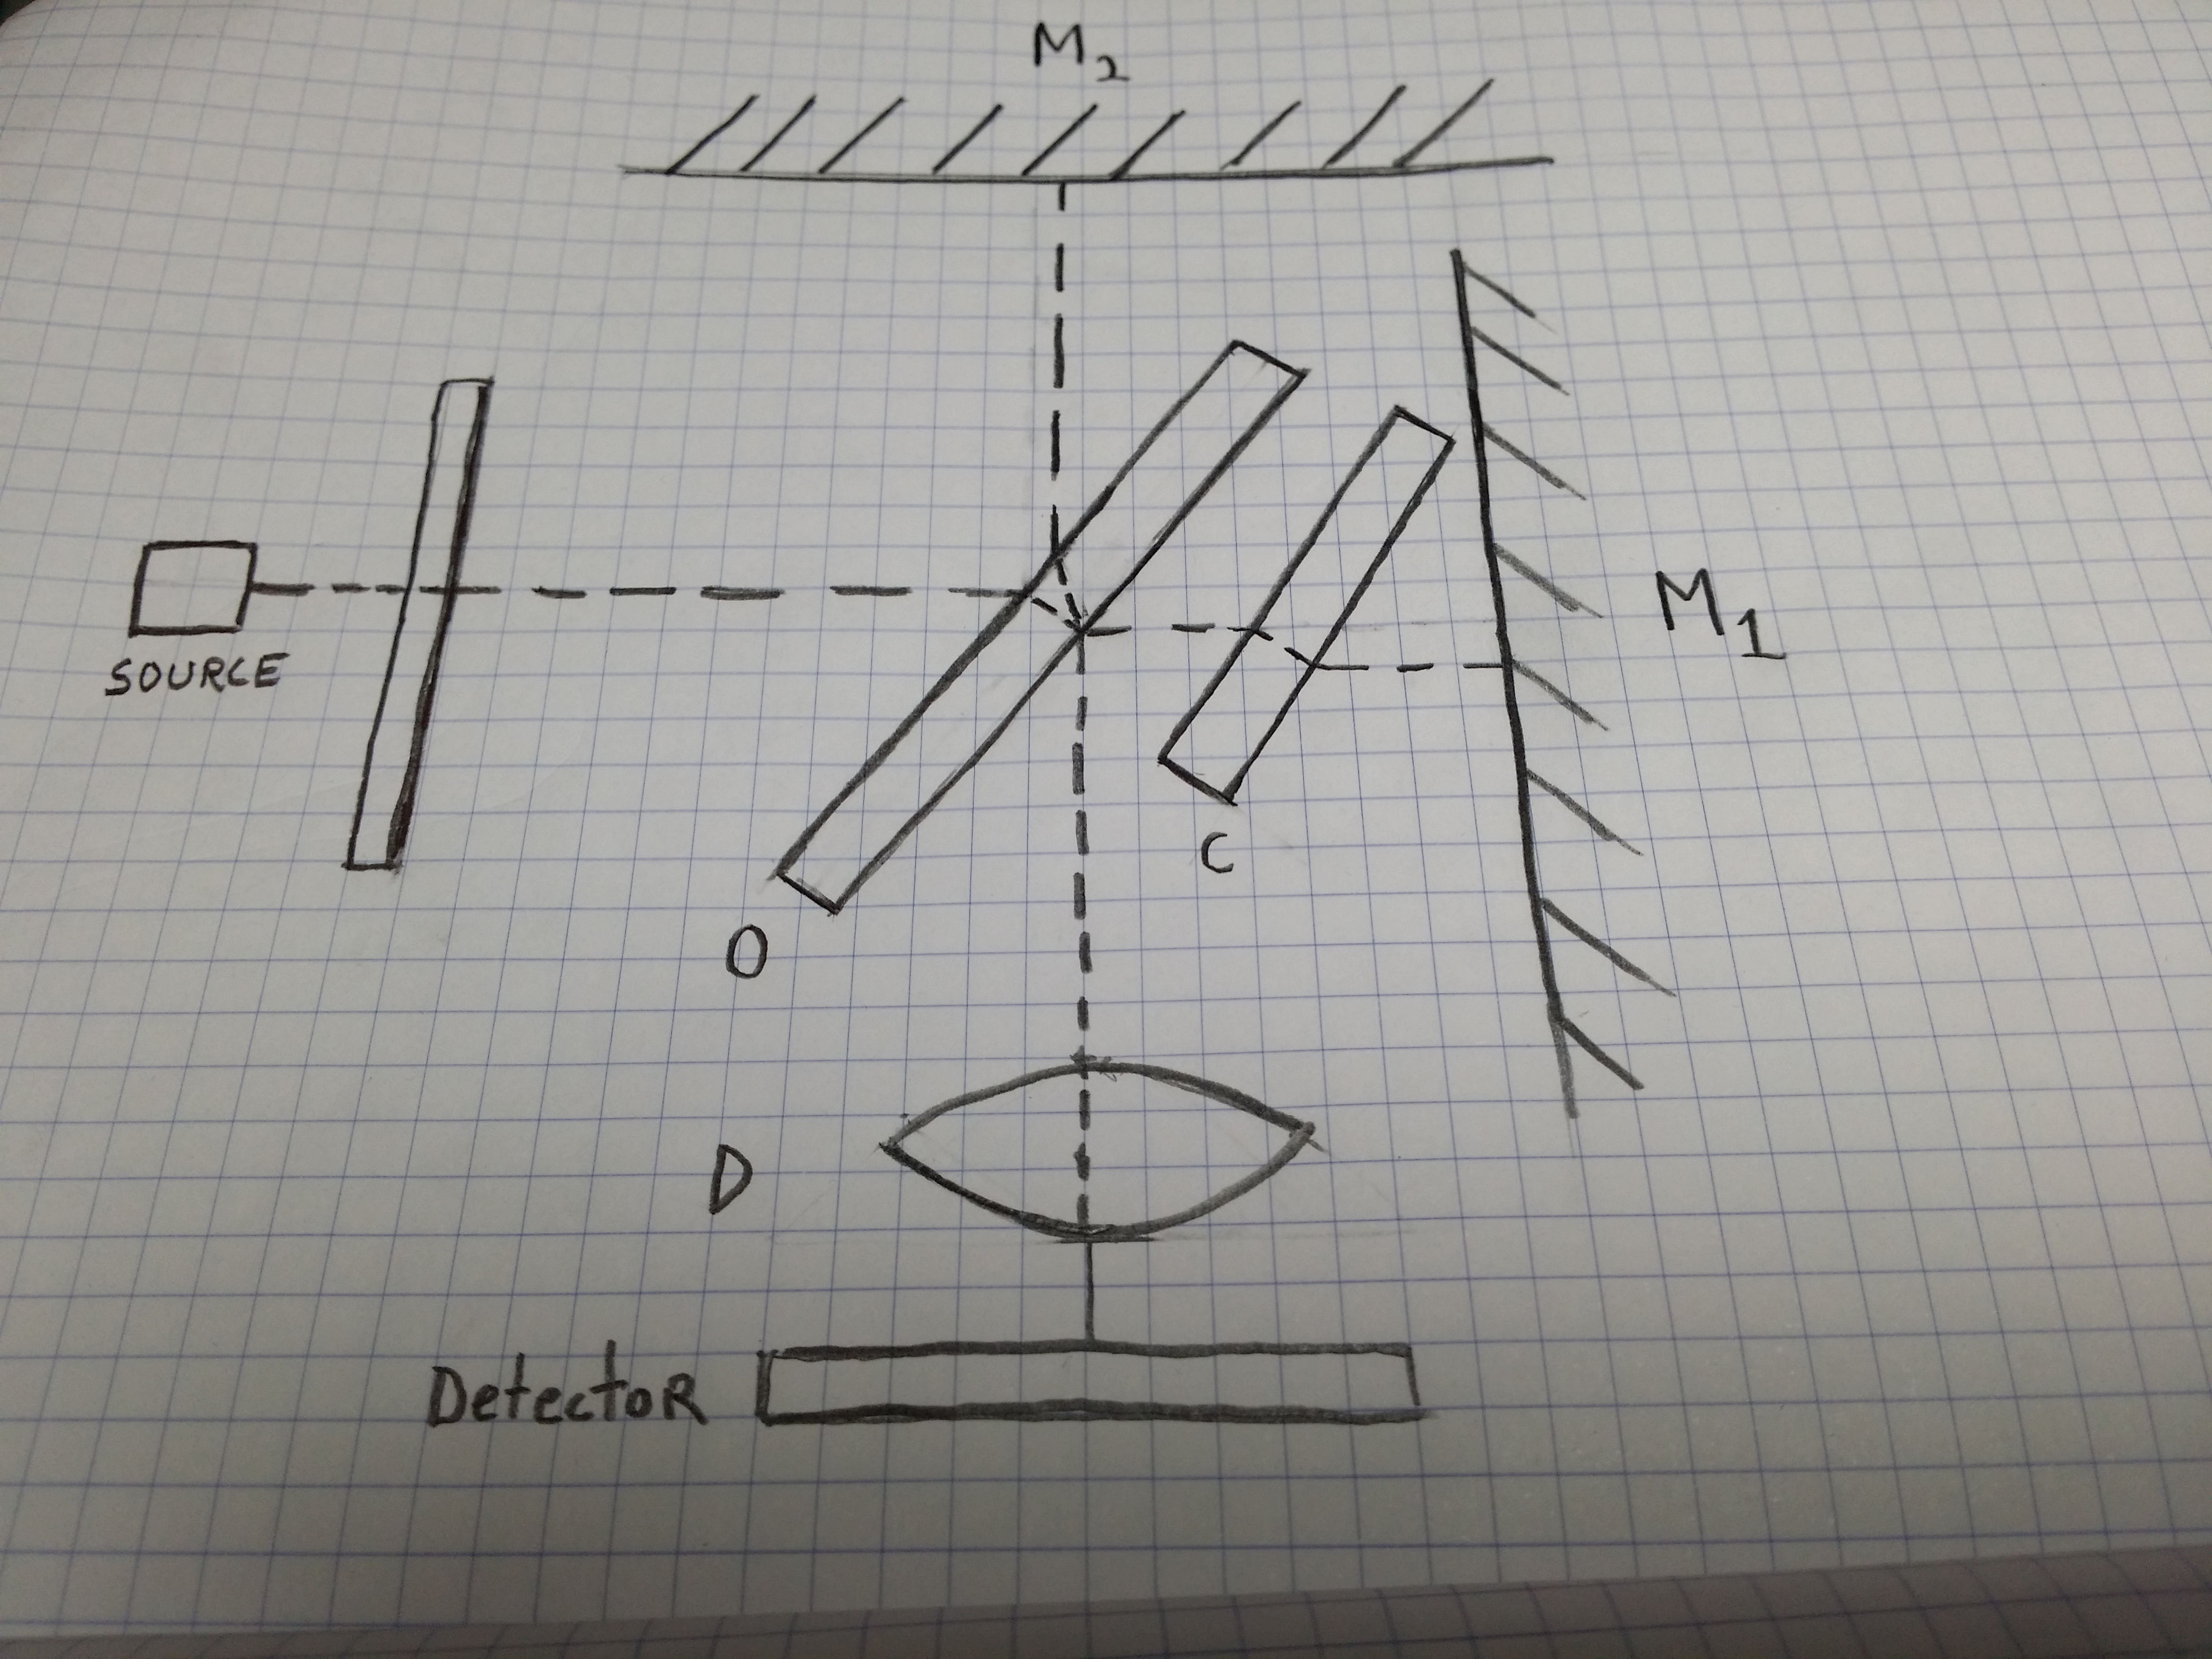
\includegraphics[scale=0.05]{/media/joe/Milarepa/Quall_Docs/tamara/figures/michaelson2.jpg}
\end{figure}
 Light travels from the \emph{source} into a beam-splitter $O$, at an angle. The beam is partially reflected and partially transmitted. The reflected component travels to mirror $M_1$ and the transmitted component to mirror $M_2$. Both beams are reflected by their respective mirrors straight back into the beam-splitter, where one component of the of either wave is then projected down to the \emph{Detector}.
 
 N.B. element $C$ is a clear piece of dielectric with the same index of refraction and width as the beam-splitter $O$. It corrects for the difference in path lengths between the two beams. However, this will not correct for the additional phase term $k_0$, which is introduced as the result of internal reflection on the $OM_2$ leg, which occurs at $O$. There will also be a secondary set of beams (omitted), which will occur on the left side of $O$.\cite[p.388]{Hecht1987}
 
This implementation is still not exactly correct in theory, but after a little calibration,  This will result in a fringe pattern at \emph{Detector}, the nulls of which are fairly close to:
\begin{equation}\label{mfringe}
 2d\cos{\theta_m} = m\lambda_0
\end{equation}
where $m$ is any integer---call it the \emph{order}, $d$ is the distance between the mirrors, and $\lambda_0$ is the wavelength of the light source. The fact that the fringe diameters are wavelength-dependent is a dispersion byproduct of the beam-splitter. If the light source has multiple wavelengths present, interference still occurs. This would cause other fringes to appear at the appropriate values for $\lambda_0$.\cite[p.~388]{Hecht1987} For every component wavelength. 

If instead, we use a monochromatic source, the interference between two parallel mirrors $M_1$ and $M_2$ will consist of many concentric rings. These rings are called \emph{fringes of equal inclination}. Each ring has a fixed order, $m$, which is its distance in number of rings from the center. By counting the number of rings, we can find the number of half-wavelengths between the mirrors $M_1$ and $M_2$. As the mirrors move closer together, the order decreases, and one after another, the rings move toward the center of the bull's-eye and disappear. 
To find the angular radius of a particular ring, $p$, we use the following:\cite[p.~390]{Hecht1987}
\begin{equation}\label{haidinger}
\cos{\theta_p} \approx \theta_p = \sqrt{ \frac{p \lambda_0}{d} }
\end{equation}
where, since the rings are stationary, $\theta_p = \theta_m$. We will see a different case below. Furthermore, since we presume to look only at a small angle subtended from the detector, we can use a Taylor approximation to make the formula faster to calculate. \cite[p.~390]{Hecht1987}

If we replace $M_1$ with an arbitrary surface, we could use this as a rangefinder. It turns out that for some applications, this sort of topology works well.\cite[p.~390]{Hecht1987} Adding an attenuator on the $OM_2$ leg---now called the \emph{reference beam}---we could theoretically adjust for losses due to scattering. This will be necessary for the system to produce an interference pattern in the first place.

Keep in mind that for a wavelength $\lambda=500$ nm, and a distance $d = 10$ cm, the order $m_0$, which corresponds to the number of fringes in the pattern, will be $400,000$.
While interpreting the fringe pattern as a whole is something our eyes can do quickly, it is unreasonable to assume our detector would have the spatial resolution or frame rate necessary to do this in real time. Furthermore, it isn't necessary, as long as we decide to look at the velocity instead. 

A typical interferometer only has a single photodetector, or at most an array. A single photodetector can be used to count the number of fringes that pass over a single point, and would be able to detect the magnitude of the velocity. In general, to detect the velocity while preserving the direction, a slightly different technique is used.\cite[p.~241]{Baker1990}

The cost of building such a device as a prototype is not very high. There are potentially some optical components that would need to be well made. In particular, the mirrors would have to be of good quality, and everything would have to be mounted with finely adjustable stands. However, to construct a housing for the device would be costly.

The field-readiness of the device, as described above, is fairly low. There are 8 minimum components, counting the reference attenuator (discussed but not shown), that would each require fully locking, adjustable supports. Furthermore, unless one added additional mirrors, the maximum distance that could be measured with the device is the length of the reference beam. Therefore an arm must be constructed to house it, etc.

The quality is limited by the devices inability to discern direction of motion. The device is clearly much better suited for displacement measurements. If the fringe patterns could be analyzed more directly, it could be made to track direction, but that would necessitate a loss in frame rate, field readiness, and an increase in cost.

The device is fairly general. It can measure vibrations even on rough surfaces by calibrating the reference beam.
 \subsection{Laser Doppler Vibrometry}
 \emph{Laser Doppler Vibrometry} is an attempt to solve some of the drawbacks concomitant with Michelson or other standard interferometry methods, most importantly the sign ambiguity. \cite{Giuliani2003}
 This is typically accomplished in one of two ways. The first method is to use polarization to read instantaneous velocity in quadrature. The second is to frequency shift the reference beam by a constant value prior to mixing the beams back together.\cite{Giuliani2003}
 Since the first method is essentially just a doubling of the interferometer approach, we shall focus on the operation of the second method. The frequency shifting is performed by an acousto-optic modulator, typically a \emph{Bragg cell}. Such devices are ultrasonic piezoelectric transducers which are transparent and capable of modulating their indeces of refraction at sufficiently high frequencies to shift the color of the light by a few tens of Mhz. This is applied to the reference beam in order to produce fringe patterns that move at a constant velocity when the surface is at rest. This way, a change in the displacement in the negative direction corresponds to a negative acceleration in the fringe pattern. The bandwidth is then limited by how far down the Bragg cell can shift the reference beam frequency.\cite[p.~241]{Baker1990}
 
 Either method is guaranteed to cost a lot more, even to prototype. The quadrature method doubles the cost of the prototype, and will also increase the cost of a field version considerably. The frequency shift method requires the use of a Bragg cell, which is expensive.
 
 As for their field-readiness, the added bulk of the quadrature method is unreasonable. Furthermore, it poses even more problems related to calibration. The frequency shift method seems to be a better choice for field work out of the two. Bragg cells are not very big, and therefore portability is not any more hindered than the case of the interferometer.
 
For the quadrature method the quality is likely very good. For the frequency shift method, the quality depends on the Bragg cell, but it will be optically band-limited, due to the heterodyning process.
 
 There are many variants that have been suggested on this general idea. C.f. \cite{Pickering1986} for a good overview of early techniques, \cite{Baker1990}, and \cite{Roos1996} for more specific applications. 
 \subsection{Self-Mixing LDV}
 An especially attractive variant on the Laser Doppler Vibrometer, the \emph{Self-Mixing} LDV, uses the laser cavity itself as the location of beam mixing. Therefore, no external mirrors are required. This technique strongly suggests the use of a diode laser, although it has been attempted in tube lasers as well.\cite{Giuliani2003} Modern laser diodes frequently have a second pair of pins, which connect to the embedded photosensitive element. 
While the self-mixing approach seems to work without any accoutrements besides the laser diode and an attenuator, the dynamic range in this configuration is poor. Thus, much of the research contributing to the design of these devices is dedicated to improving them in this respect. 
Since this technique has been established for some time, some fairly sophisticated implementations exist in the literature. This technique looks very promising on all fronts. 
\end{section}

\end{chapter}
\begin{chapter}{Charles Curtis}
\begin{abstract}
 A thread running through a number of Alvin Lucier's early works seems to be an urge to equate musical performance with an act of scientific observation, or measurement. With sound, room acoustics, and various corollaries of sound as the declared objects of this observation, Lucier seems to put musicians and listeners in a shared encounter with ``nature'' and ``the natural world'' that combines elements of science, mysticism and universalism. What are the sources of these notions of ``nature'' and art-making, and what is the context in post-World War II America that gives rise to this interest in measuring the behavior of sound as an aesthetic? What conclusions can be drawn from the language, methodologies and idea-world that Lucier makes use of?
\end{abstract} 
\begin{section}{Prologue}
 Some of Alvin Lucier's pieces from the 70's suggested a complex relationship to the scientific method. Through the use of this imagery in performance, he offers to the listener an experience of the objective, which is unknowable, and therefore transcendent. He achieves this through the act of labored, meticulous exploration and observation. Embedded in these themes is a mystical tension between nature and measurement, which seems to emerge in his early work as the result of his personal solution to the contradictory assumptions of modernity.

In turning our attention to measuring the extensional world as an aesthetic object, Lucier's music tells ghost stories. At some point, the signifiers of frank, stark inquiry---unadorned, precise, a little nerdy---evaporate, with dropplets of ectoplasm, into the sublime holism of the absolute. The listener is faced with a transformation of the everyday into the the timeless, and a process that carries itself quite similarly to scientific inquiry is the source of this transformation. 
\end{section}
\begin{section}{Method}
 Some scholars have noted that Alvin Lucier's musical ideas occasionally revolve around images, rather than sounds.\cite{kuivila2012}This use of the word connotes less a reliance on sight, per se, than situations: Lucier immediately references the image of the whistler station at the opening of \underline{Gravity's Rainbow}, for example, in reminiscing about the inspiration for ``Sferics.''\cite[p.~151]{lucier2012} His early text-scores, too, are saturated with visual and narrative imagery: for example, the notation for ``The Queen of the South,'' is about as visually overstimulating as any of Pynchon's scenery-filled, high-speed, run-on sentences.\cite[350-352]{lucier1995} James Tenney astutely points out the Whitmanesque quality shared by much of this text.\cite[p.~16]{lucier1995}

In response, Lucier denies any frivolity: ``I'm trying to write clear linear prose that describes a complete situation, that has balance''\cite[p.~16]{lucier1995} This does not come as a surprise. Lucier, like many in his generation within the American experimental school, values clear communication over florid embellishments, perhaps in reaction to perceived tendencies concomitant with the European avant-garde. A common signifier of belonging to this subculture, at least for Lucier's generation, is to minimize grandiose self-expression. In an interview, Lucier explains the function of the text-score further, but noticeably absent is any mention of the imagery embedded into those instructions.\cite[p.~138]{lucier1995}

Rather than locating the statements and endeavors of these artists within the context that evoked them, it may be tempting to claim that Lucier actually succeeded in erasing cultural reference from his music altogether. This claim revolves around Lucier's preoccupation with scientific and natural processes.\cite{yang2012} However, to claim this would require that we ignore exactly those things which make his work unique. The fact that Lucier himself occasionally corroborates this hypothesis with statements about his own work indicates more clearly the cultural narrative that envelopes him. It does not give this claim any sort of veracity in the historiographical sense of the word: by attempting to remove cultural specificity from his work, he is actively navigating a particular cultural dialog. 

Lucier cannot help but be a great writer. His early pieces are overflowing with coherent, beautifully executed imagery, which strongly imply elements of his own character. The question, then, should not be whether Lucier's work participates in a system of signification, but rather, what is that system? It seems reasonable, given his propensity for storytelling, to derive the answer from the sorts of stories he tells. In so doing, one must be careful to locate the elements which make up the story. That is, to answer any sort of question about the man's work will require an analysis of how he positions himself---the protagonist of his own narrative---in relation to others. It will be especially illuminating to highlight the network of experiences and exchanges that have influenced him, either positively or negatively. 

This is not done in a glib attempt to stand beyond history and scoff at the failed pursuits of those who came before. On the contrary, this is intended as a nod to the man whose music, stories, and example truly inspired the author. Foucault writes, in the affected voice of the historian: "No past is greater than your present, and, through my meticulous erudition, I will rid you of your infatuations and transform the grandeur of history into pettiness, evil, and misfortune,"\cite[p.~91]{Foucalt1984} meaning to point out the shameless astigmatism such whig analyses offer. An honest account of Lucier's work---and the least insulting---must (without grovelling!) take into account the complex system of influences and reactions that are the food of the artist. In short, what was Lucier eating, and how did it find expression in his work?

To offer a complete answer to this question is, of course, impossible. Furthermore, it is a bit misguided. Instead, the author will attempt to unpack a small subset of themes, to which a small subset of Lucier's output relates. Care will be taken not to assume either opposing birds-eye-views of the polemicist or the sycophant. Care will also be taken to step back and recall that the pieces described herein represent contingent moments in the development of an artist who is still active. Some of these themes come from work Lucier made thirty years ago. Therefore the perspective I take will be dusty, limited, and subtle. 
\end{section}
\begin{section}{Alvin}
 Lucier is very fond of reminding his students that Ives sold insurance for a living. In fact, this characterization of Ives makes up the first chapter in his recent book. Ives, in Lucier's worldview, is an American solution to the problem of high Modernism, as posed by the European avant-garde.\cite[p.~3]{lucier2012} It is not difficult to imagine that Lucier might feel a kindred sort of bond, or perhaps even a line of descent. The protagonist, in Lucier's implied narrative, is not a hero, or a virtuoso, or a technician. This person is no ``courtly muse,'' to quote Emerson, via Lucier. In fact, he just might be an insurance salesman.\cite[p.~3]{lucier2012} 

An unpretentious earnestness pervades the imagery of his often vividly visual compositions. As Tenney notes in the aforementioned piece, ```plain' and `poetic' are not necessarily mutually exclusive qualities.''\cite[p.~16]{lucier1995} As a result, his compositions are simple, but not sleek. This is by design: foremost in Lucier's value system is an integral devotion to the process. He is paying Cage a rather high compliment when he says: ``he's extremely meticulous with his scores. He doesn't cheat, either.''\cite[p.~11]{lucier2012} 

Like many artists in his camp, he constantly renegotiates a balance between the desire to polish his work and the desire to allow the process to unfold on its own. For Lucier, the distinction is simultaneously one of aesthetics and one of ethics. Speaking about a recording of ``Music on a Long Thin Wire,'' where he grappled with his instinctive desire to edit, he relates: ``I said to myself, `Don't cheat. You said you wouldn't cheat. The listener may not know you cheated, but you'll know.'''\cite[p.~530]{lucier1995} 
\end{section}
\begin{section}{Nature}
If we momentarily set aside some of his more psychologically-driven entries, Lucier's early work is often positioned as an encounter with the natural: the physical, the causal, the salient. Nature, in this sense, is not limited to the domain of the pastoral landscape, but the lattice of observable facts, presented in a simple, understated tone of voice, from the reference frame of the individual. 

Furthermore, many of these compositions seem to appropriate imagery from nineteenth-century \emph{naturphilosophie} and transcendentalism. This imagery appears in the form of his text-score instructions to the performers as well as the theatrical spectacle they present to the audience. Lucier's methods, language, and imagery appear to stem from an appeal to the natural as a solution to the aesthetic contradictions set in place by modernity. 

Frequently, the enlisted performer must participate in an action of embodied measurement. Located within the already loaded space of the concert hall, these measurements function in a manner similar to virtuosic instrumental performance, in that successfully completing such an action requires the performer to commit unflinchingly to a theatrical situation, and this commitment invites the audience to observe the process as it unfolds. However, the actions completed on stage often lie outside the canonical domain of musical production. This practice of recontextualizing the non-musical, which is not uncommon in the music of the American experimental movement, might be succinctly described as “reframing.”\cite{dewar2012} By encouraging performers and audience members to relate to nature through the task of measurement, he presents nature as a basis of facts: shared, absolute, and direct. 

In the years following World-War II, a common characteristic within the subculture of the American experimental movement was a hunger for the inception of an identity separate from Europe. Lucier was no exception to this. In the opening lines of his book, \underline{Music 109}, he writes: "When I went to college we studied the masterpieces of European music... one felt one's spiritual home was in Europe...We all had inferiority complexes." \cite[p.~1]{lucier2012}

In its polemical form, this identity crisis manifested itself as a criticism of indulgent self-expression in Europe. Each composer in this group offers unique strategies for navigating this. For example, Lucier explains Cage's method of indeterminacy as a solution: ``Indeterminacy gets personal preference out of the compositional process. Isn't that a shocking idea? Weren't we always taught that art was about self-expression?''\cite[p.~11]{lucier2012} He similarly praises Christian Wolff's solution through interaction and contingency.\cite[p.~46]{lucier2012} Likewise, early Lucier relinquishes composerly control in a different way from either of these colleagues. Lucier's solution was to supplant his own conscious intelligence with the intelligence of nature. 

Although he might use less sentimental vocabulary to describe it, the idea of a natural intelligence is central to the construction of nature in Lucier's early work. He expresses an affinity for this concept in several ways. Perhaps most obvious is his devotion to his self-ascribed role as a documentarian of this intelligence. Many of Lucier's compositions from this period seem to consist of the unadorned presentation of a physical or biological principle. 

According to Lucier, this is the best method of contemplating the natural, and learning whatever it has to offer: ``I don't bring an idea of mine about composition into a space and superimpose it on that space, I just bring a very simple idea about a task that players can do and let the space push the players around. In that way, I always learn something about a space...''\cite[p.~78]{lucier1995} In the interview from which the above quote was taken, Lucier was talking about \emph{Vespers}, a piece that involves sound in spaces, but one could easily imagine him saying something analogous about any of the processes his early pieces explore. Thus, space is simultaneously granted agency and intelligence.  
\end{section}
\begin{section}{Notes on the Scores}
 \subsection{Vespers (1968)}

The text-score for ``Vespers'' includes a brief homage to ``...all living creatures who inhabit dark places and who, over the years, have developed acuity in the art of echolocation.''\cite[p.~312]{lucier1995} In particular, he is referring to the common North American bat.\cite[p.~86]{lucier2012} 

The piece first calls for players to blind themselves, either with blindfolds or sunglasses, or by performing in the dark. Lucier delineates that the performers should use specialized clicking devices, called \emph{Sondols}, which were constructed by an acquaintance of his. These devices were designed to allow humans to communicate with dolphins.

He goes on to ask the performer to ``accept and perform the task of acoustic orientation by scanning the environment and monitoring the changing relationships between the outgoing and returning clicks.''\cite[p.312]{lucier1995} His description of the piece is largely pragmatic, but towards the end he includes a few lines of simple, evocative, prose:
``Dive with whales, fly with certain nocturnal birds or bats... or seek the help of other experts in the art of echolocation.''\cite[p.~314]{lucier1995}


\subsection{The Queen of the South (1972)}

The text-score for this piece attributes its inspiration to the work of two individuals: Ernst Florens Friedrich Chladni, and Hans Jenny. The first volume of Jenny's book, "Cymatics," which had just been published in 1967, combined absolutely stunning color photographs of phenomena produced by vibration. Jenny's work was also heavily influenced by Chladni, who in the early 19\textsuperscript{th} century became famous because of his methods for visualizing acoustic modes. Jenny passed away the year Lucier wrote the piece. 

In his interview about the piece in ``Reflections,'' he gives no clues about the rich imagery he embeds into his score, which is consistent with his remarks to Tenney. Regardless, in the text, Lucier gives us the setting, with a whimsical tone of voice that reflects what is probably earnest excitement. The list is almost alchemical in its word choice: 

\begin{singlespace}
``Sing speak or play electronic or acoustic musical instruments in such a way as to activate metal plates, drum heads, sheets of glass, or any wood, copper, steel, glass, cardboard, earthenware, or other responsive surfaces upon which are strewn quartz sand, silver salt, iron filings, lycopodium, granulated sugar, pearled barley or grains of other kinds, or other similar materials suitable for making visible the effects of sound.''
\end{singlespace}

Here, he is echoing many of the elements Jenny catalogs, in the pages of ``Cymatics,'' to describe his methods.\cite{Jenny2001} The longest paragraph in the score informs us that we have a choice: we could either improvise with the system, or we could follow the imagery that results from the sound.
\end{section}
\begin{section}{Ernst}\label{chladni}
 It was not until 1786, four years after his father died, that Chladni began lecturing on acoustics. He had spent those four years tackling open problems in the field: "...I performed experiments on transversal [sic] vibrations of rods, which had been the subject of theoretical studies of Leonhard Euler and Daniel Bernoulli, and then on the vibrations of plates, which were an unknown field."\cite[p.~27]{Ullmann2007} Chladni had also begun building novel instruments, largely inspired by the glass harmonica, which he had read about in a publication by Nicolaus Forkel. This also convinced him to use a bow to excite the resonances in his objects, rather than merely exciting them with tapping.\cite[p.~27]{Ullmann2007}

He had also read about the experiments of Georg Christoph Lichtenberg, who in 1777 had become famous for his experiments with electricity. Lichtenberg created strikingly beautiful, spidery figures by sprinkling various powders onto dielectric plates and applying current into them. When Chladni attempted this, however, an entirely different sort of pattern emerged. These would come to bear his name.\cite[p.~27]{Ullmann2007}

Chladni meticulously documented and cataloged the patterns he found. For his first book, published in 1787, he included drawings of the patterns which emerged on each of the 11 plates he investigated. There were 166 of these figures total. This book, \emph{``Entdeckungen uber die Theorie des Klanges''}, provided empirical evidence which conflicted with Euler and Golovin's mathematical models of rigid plates. At the end of the book, he reiterated the open mathematical questions concomitant with constructing a new model.\cite[p.~27]{Ullmann2007}

Meanwhile, Chladni had effectively run out of money. His infrequent, part-time status as a guest lecturer barely made the man enough to support himself.\cite[p.~27]{Ullmann2007} He decided to go on tour. He recalls, 
``It occurred to me that an artist who knows how to give himself some publicity is less attached to a certain place and has more opportunities of being received kindly and profiting nearly everywhere than a scholar dedicated to the academic life, and I hoped to succeed likewise, not by means of virtuosity, because I had so late in life begun to learn music, but due to the invention of a new instrument.''\cite[p.~17]{Stockmann2007}

From 1792 - 1812 he traveled Europe, giving demonstrations of his findings.\cite[p.~21]{Stockmann2007} Early in his travels he met Lichtenberg, and their interaction sparked his interest in meteors, which, much later in life, would become the topic of his second contribution to the scientific community.\cite[p.~28]{Ullmann2007} It is clear from his remarks that Chladni situated his findings as similar to, but distinct from, musical virtuosity. He invented two novel musical instruments, both of which failed to capture the public imagination nearly as effectively as his plate demonstrations. Because of the physical immediacy and synaesthetic spectacle of his demonstrations, Chladni was able to present his lectures in a way that appealed to wealthy, powerful people all across Europe. 

Although he was content not to speculate beyond the results of his observations, this could not prevent others from speculating for him.\cite[p.~13]{Bonds2012} The possibility that nature could provide the basis for ideas surrounding musical and visual beauty especially resonated with the \emph{Naturphilosophen} in Germany, and later the Transcendentalists in America.\cite[p.~15]{Bonds2012} Goethe, for example, initially paints him as pragmatic to a fault. In a letter to Schiller dated 1803, Goethe writes: 

``[Chladni] belongs to... those blissful persons who have not the faintest idea that there is something as \emph{naturphilosophie} and who are only attentively trying to observe phenomena, which they will then classify and make use of...''\cite[p.~18]{Stockmann2007}

In other words, Chladni seemed a lot like an insurance salesman.

Goethe later recognized similarities between the patterns Chladni found and other patterns in nature, in particular, Johann Seebeck's work with polarized light. Goethe believed this to be proof that there was an underlying principle connecting the two phenomena, and, by extension, all phenomena.\cite[p.~17]{Bonds2012} Later, perhaps once Chladni's contributions in other areas of inquiry became evident, Goethe would praise Chladni: ``...an ingenious man feels the impetus to study two natural phenomena which are far away from each other, and investigates both of them continuously.''\cite[p.~31]{Ullmann2007}

Word of Chladni's experiments also had a profound effect on Ralph Waldo Emerson, who believed the symmetrical, undulating patterns he had found represented a portal to the supernatural. As such, Chladni's plates proved that an experience of the transcendent could be achieved through music: ``Orpheus, then, is no fable: Sing, and the rocks will crystallize; Sing, and the plants will organize.''\cite[p.~15]{Bonds2012}

Furthermore, it is reasonable to believe there are certain themes---regardless of their veracity---in the story of Chladni that must have made him especially heroic to some. He was essentially a self-made man, who not only worked outside of the accepted realm of a natural scientist, but thrived there. 

Finally, we can approach the puzzling case of Dr. Hans Jenny. It is difficult to find anything of credible substance on the man. Perhaps this fact speaks more to the chauvinism of the academy---the author included---than anything else: Jenny certainly seems to have a lot of supporters, and not very many biographers. His own books are readily available, however, and the two volumes of \underline{Cymatics} paint a rather bizarre picture.

``However natural these things may seem, they are.[sic] in fact,
 not. It must be realized that this periodicity represents an aspect of the world, and at first its mysteriousness always inspires a feeling of the greatest astonishment.'' \cite[p.~16]{Jenny2001}

The book's eponymous thesis states, roughly, that the entire world is made up of waves, having momentarily paused a torrent of terms related to cellular tissue and organs and organelles. The book itself is a collection of masterfully taken photographs of phantasmagoria, in the illustration of the vast interconnected system of universal principles. He makes enormous lists of only somewhat categorized phenomena, using contrast between the items to convey the breadth of his theories. He is almost always pictured surrounded with scientific equipment. 
\end{section}
\begin{section}{Cause and Effect}
 Lucier's natural intelligence cannot be properly interpreted by human intelligence. In order to gain an understanding of it we must contemplate it directly, without bias. When the aspect of nature Lucier wants to frame cannot be directly perceived, technology must serve as a mediator. Categorically a product of human intelligence, however, technology can only translate natural intelligence if it is unbiased. 

Therefore, Lucier frequently makes the claim that the tools employed in his early compositions are intended to be prosthetics of the sensory organs, and not musical instruments: ``Acoustical test equipment is, by its very nature, free of content. What goes into a material or environment to be tested must be neutral so that the results are unbiased.''\cite[p.~456]{lucier1995} The activities permitted by this method of knowing must fall short of aesthetic interpretation in order to be acceptable. He describes the appropriate examples of contemplation of the natural as ``testing, probing, exploring.''\cite[p.~440]{lucier1995} In a word: measurement.

The word ``measurement,'' in this context, does not precisely connote other possible uses of the term. E.g, measurement does not mean the same thing to Lucier as it did to Cage. Lucier makes this very clear in the accounts of his own work and that of his colleague's. According to Lucier, and to Cage himself, Cage's work often uses measurement as a means to construct the experience of acausality. As a result, the Cagean measurement typically quantifies its results, so they can be made illegible through incongruous translation. 

By contrast, the measurements permitted by Lucier's early compositions are frequently qualitative, and more concerned with observation: ``My pieces are cause and effect whereas Cage's are not. ... I don't get in the middle and destroy the relationship.''\cite[p.~230]{lucier1995} Perhaps this explains why, for example, Lucier never specifies numerical measurements for "Music on a Long Thin Wire." Because his object is the natural intelligence latent in the physical system, with all its particular eccentricities, Lucier's early work privileges certain forms of measurement over others. This is because Lucier was playing with the notion of the legitimacy of scientific modes of observation. His early compositions seem to propose that the forms of measurement afforded by scientific observation alone are sufficient to achieve transcendence. To ``get in the middle'' would suggest that one is no longer observing the system in its natural state. 

Tellingly, Lucier describes the process of arriving at ``Vespers'' as a process of looking outside.\cite[p.84]{lucier2012} At this point in his aesthetic development, the measurement of the natural world provides him a way to escape his own expectations. The exploration of space in the context of  ``Vespers'' brings us into a direct experience of the life of a space. Furthermore, ``Vespers'' brings its performers a state where they must contend with the task of being so restricted. As a composition, the piece is typical for the way Lucier's early works use measurement- there is no guide, no organizing principle, not even a singular \emph{ending}. 

The role of science in our culture seems to have changed in the last few decades. Bruno Latour puts it succinctly: "Scientists no longer appear as a voice from nowhere mysteriously fused with the undisputable[sic] necessity of matters of facts." \cite{Latour2011} These days, many of us have come to accept that science is no longer apolitical, if it ever had been in the first place. Underscoring the assumption of the neutrality of scientific measurement is the commonly excepted belief that we, who have developed cities, are modern, and therefore removed from nature entirely. Of course, this has never been the case.

Later in his career, Lucier would move away from signifiers of science as a method for legitimizing his characteristic exploratory measurements. Since the 80's, his work has become more indicative of a deep appreciation for the Western Tradition. This reconciliation could only come about because of the process he went through in the 70's, of turning away from his "Bach, Beethoven, and Brahms,"\cite[p.~1]{lucier2012} to develop a separate narrative, populated with characters who, in all likelihood, all sell insurance for a living.
\end{section}

\end{chapter}
\begin{chapter}{A Proposed \\Mode-Solver: Assessment}
 \begin{section}{Experiment Results}\label{sec:exp_results}
An initial set of experiments was undertaken to test the validity of the algorithm described in \ref{sec:modesolver}, and the conditions for convergence of the eigenfrequencies. Multichannel audio signals were synthesized using all-pole filters and white noise. The activations of the eigenfrequencies were randomly distributed across the channels for each signal. This was intended to simulate the coupling between mode shape and measurement location, which must be assumed to be unknown, therefore random. The signals could simulate a number of damping regimes by varying the distributions of the magnitudes of the poles. 

A total of 20 parameter states were tested with 2 trials for each state. The stimuli were each 1000 samples long, with 4 channels of data. The two parameters that varied were the damping regimes and number of modes in the stimulus. 

The stimuli were grouped by the magnitudes of their poles into 10 ranges varying from 0-10\%, 10-20\%, 20-30\%, and so on. The stimuli were further divided into 2 groups: one which exhibited 24 modes, the other which exhibited 28. The mode solver always attempted to find 24 eigenfrequencies.

The resulting eigenvalue sets were plotted against each other on the complex plane for each trial. Overall, the results suggest the mode solver performs better at finding modes which are less damped, which is fairly consistent with the findings of others. \cite{Chen2012} \cite{Feeny1998} \cite{Kerschen2002} \cite{Han2003} 

The mode solver was also asked to plot the mode shapes as complex contours. Since the stimulus model did not explicitly specify these, they cannot be verified against any data. They just look pretty.

N.B., this algorithm does not suffer from the negative effects of mean-subtraction as referenced in \cite{Chen2012}, and above in section \ref{sec:modes_other}. Our method subtracts the mean of the entire data set from each point in the data set, then it breaks the entire data set into smaller matrices of length $kb$, spaced one sample apart, and proceeds with the DMD on each of those blocks. therefore, each submatrix is not re-centered, but rather permitted to drift on timescales much larger than $k$.

Therefore the frequency-domain distortions associated with the DFT, i.e. arranging the poles at evenly spaced intervals around the unit circle, will not occur. This technique's behavior, like that of DMD---and presumably other least-squares prediction methods---converges on DFT-like behavior as the time-series order, $k$, approaches the time-series length of dataset, $n$. Thus there appears to be a compromise between the number of modes this type of system can find, and the accuracy. Since we do not perform mean-subtraction across column vectors of $X$, this is perhaps another reason to use wider, rather than longer, datasets. However, this is just speculation at the moment.

Future tests will attempt to find the effects of increasing the number of channels. This will require a different implementation of the stimulus synthesizer. Other aspects of future work include verifying the forcing function estimation and mode shapes. 

In the complex plots below, the stimulus poles are plotted in red, while the algorithm's 24 estimation poles are plotted in blue. The first block of stimuli had 24 modes, and the second block had 28. These plots are ordered by increasing polar magnitude (or decreasing damping).

The complex contour plots of the modes, which begin on page \pageref{fig:mode_contours} of this chapter, describe the mode shapes as they are expressed across each of the four channels, for six samples (in time) each. The real contours are placed above the imaginary contours. Only block 1, trial 1, pass 1 is printed.
\begin{singlespace}
\begin{figure}[h]
\includegraphics[scale=0.25]{/media/joe/Milarepa/Quall_Docs/miller/experiments/new_exp/05/trial01/figures/poles}
\includegraphics[scale=0.25]{/media/joe/Milarepa/Quall_Docs/miller/experiments/new_exp/06/trial01/figures/poles}
\caption{(above) block 1, trial 1, passes 1 \& 2}
\includegraphics[scale=0.25]{/media/joe/Milarepa/Quall_Docs/miller/experiments/new_exp/05/trial02/figures/poles}
\includegraphics[scale=0.25]{/media/joe/Milarepa/Quall_Docs/miller/experiments/new_exp/06/trial02/figures/poles}
\caption{(above) block 1, trial 2, passes 1 \& 2}
\end{figure}
\begin{figure}[h]
\includegraphics[scale=0.25]{/media/joe/Milarepa/Quall_Docs/miller/experiments/new_exp/05/trial03/figures/poles}
\includegraphics[scale=0.25]{/media/joe/Milarepa/Quall_Docs/miller/experiments/new_exp/06/trial03/figures/poles}
\caption{(above) block 1, trial 3, passes 1 \& 2}
\includegraphics[scale=0.25]{/media/joe/Milarepa/Quall_Docs/miller/experiments/new_exp/05/trial04/figures/poles}
\includegraphics[scale=0.25]{/media/joe/Milarepa/Quall_Docs/miller/experiments/new_exp/06/trial04/figures/poles}
\caption{(above) block 1, trial 4, passes 1 \& 2}
\end{figure}
\begin{figure}[h]
\includegraphics[scale=0.25]{/media/joe/Milarepa/Quall_Docs/miller/experiments/new_exp/05/trial05/figures/poles}
\includegraphics[scale=0.25]{/media/joe/Milarepa/Quall_Docs/miller/experiments/new_exp/06/trial05/figures/poles}
\caption{(above) block 1, trial 5, passes 1 \& 2}
\includegraphics[scale=0.25]{/media/joe/Milarepa/Quall_Docs/miller/experiments/new_exp/05/trial06/figures/poles}
\includegraphics[scale=0.25]{/media/joe/Milarepa/Quall_Docs/miller/experiments/new_exp/06/trial06/figures/poles}
\caption{(above) block 1, trial 6, passes 1 \& 2}
\end{figure}
\begin{figure}[h]
\includegraphics[scale=0.25]{/media/joe/Milarepa/Quall_Docs/miller/experiments/new_exp/05/trial07/figures/poles}
\includegraphics[scale=0.25]{/media/joe/Milarepa/Quall_Docs/miller/experiments/new_exp/06/trial07/figures/poles}
\caption{(above) block 1, trial 7, passes 1 \& 2}
\includegraphics[scale=0.25]{/media/joe/Milarepa/Quall_Docs/miller/experiments/new_exp/05/trial08/figures/poles}
\includegraphics[scale=0.25]{/media/joe/Milarepa/Quall_Docs/miller/experiments/new_exp/06/trial08/figures/poles}
\caption{(above) block 1, trial 8, passes 1 \& 2}
\end{figure}
\begin{figure}[h]
\includegraphics[scale=0.25]{/media/joe/Milarepa/Quall_Docs/miller/experiments/new_exp/05/trial09/figures/poles}
\includegraphics[scale=0.25]{/media/joe/Milarepa/Quall_Docs/miller/experiments/new_exp/06/trial09/figures/poles}
\caption{(above) block 1, trial 9, passes 1 \& 2}
\includegraphics[scale=0.25]{/media/joe/Milarepa/Quall_Docs/miller/experiments/new_exp/05/trial10/figures/poles}
\includegraphics[scale=0.25]{/media/joe/Milarepa/Quall_Docs/miller/experiments/new_exp/06/trial10/figures/poles}
\caption{(above) block 1, trial 10, passes 1 \& 2}
\end{figure}
\begin{figure}[h]
\includegraphics[scale=0.25]{/media/joe/Milarepa/Quall_Docs/miller/experiments/new_exp/07/trial01/figures/poles}
\includegraphics[scale=0.25]{/media/joe/Milarepa/Quall_Docs/miller/experiments/new_exp/08/trial01/figures/poles}
\caption{(above) block 2, trial 1, passes 1 \& 2}
\end{figure}
\begin{figure}[h]
\includegraphics[scale=0.25]{/media/joe/Milarepa/Quall_Docs/miller/experiments/new_exp/07/trial02/figures/poles}
\includegraphics[scale=0.25]{/media/joe/Milarepa/Quall_Docs/miller/experiments/new_exp/08/trial02/figures/poles}
\caption{(above) block 2, trial 2, passes 1 \& 2}
\end{figure}
\begin{figure}[h]
\includegraphics[scale=0.25]{/media/joe/Milarepa/Quall_Docs/miller/experiments/new_exp/07/trial03/figures/poles}
\includegraphics[scale=0.25]{/media/joe/Milarepa/Quall_Docs/miller/experiments/new_exp/08/trial03/figures/poles}
\caption{(above) block 2, trial 3, passes 1 \& 2}
\includegraphics[scale=0.25]{/media/joe/Milarepa/Quall_Docs/miller/experiments/new_exp/07/trial04/figures/poles}
\includegraphics[scale=0.25]{/media/joe/Milarepa/Quall_Docs/miller/experiments/new_exp/08/trial04/figures/poles}
\caption{(above) block 2, trial 4, passes 1 \& 2}
\end{figure}
\begin{figure}[h]
\includegraphics[scale=0.25]{/media/joe/Milarepa/Quall_Docs/miller/experiments/new_exp/07/trial05/figures/poles}
\includegraphics[scale=0.25]{/media/joe/Milarepa/Quall_Docs/miller/experiments/new_exp/08/trial05/figures/poles}
\caption{(above) block 2, trial 5, passes 1 \& 2}
\includegraphics[scale=0.25]{/media/joe/Milarepa/Quall_Docs/miller/experiments/new_exp/07/trial06/figures/poles}
\includegraphics[scale=0.25]{/media/joe/Milarepa/Quall_Docs/miller/experiments/new_exp/08/trial06/figures/poles}
\caption{(above) block 2, trial 6, passes 1 \& 2}
\end{figure}
\begin{figure}[h]
\includegraphics[scale=0.25]{/media/joe/Milarepa/Quall_Docs/miller/experiments/new_exp/07/trial07/figures/poles}
\includegraphics[scale=0.25]{/media/joe/Milarepa/Quall_Docs/miller/experiments/new_exp/08/trial07/figures/poles}
\caption{(above) block 2, trial 7, passes 1 \& 2}
\includegraphics[scale=0.25]{/media/joe/Milarepa/Quall_Docs/miller/experiments/new_exp/07/trial08/figures/poles}
\includegraphics[scale=0.25]{/media/joe/Milarepa/Quall_Docs/miller/experiments/new_exp/08/trial08/figures/poles}
\caption{(above) block 2, trial 8, passes 1 \& 2}
\end{figure}
\begin{figure}[h]
\includegraphics[scale=0.25]{/media/joe/Milarepa/Quall_Docs/miller/experiments/new_exp/07/trial09/figures/poles}
\includegraphics[scale=0.25]{/media/joe/Milarepa/Quall_Docs/miller/experiments/new_exp/08/trial09/figures/poles}
\caption{(above) block 2, trial 9, passes 1 \& 2}
\includegraphics[scale=0.25]{/media/joe/Milarepa/Quall_Docs/miller/experiments/new_exp/07/trial10/figures/poles}
\includegraphics[scale=0.25]{/media/joe/Milarepa/Quall_Docs/miller/experiments/new_exp/08/trial10/figures/poles}
\caption{(above) block 2, trial 10, passes 1 \& 2}
\end{figure}
\begin{figure}[h]\label{fig:mode_contours}
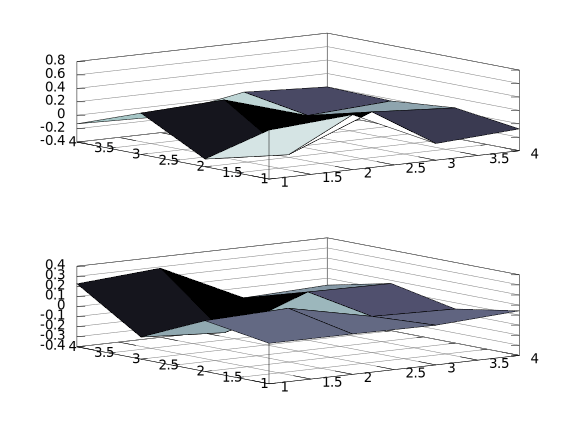
\includegraphics[scale=0.35]{/media/joe/Milarepa/Quall_Docs/miller/experiments/new_exp/05/trial10/figures/mode01}
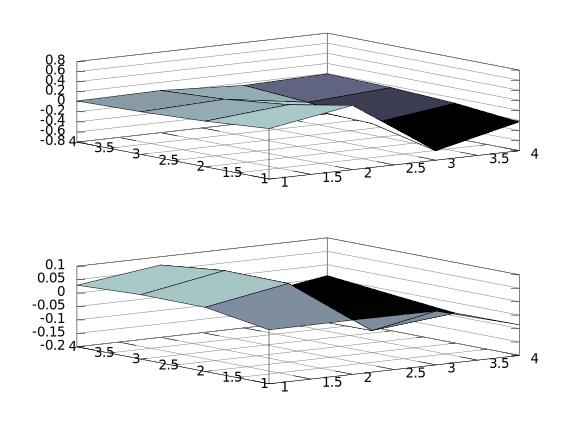
\includegraphics[scale=0.35]{/media/joe/Milarepa/Quall_Docs/miller/experiments/new_exp/05/trial10/figures/mode02}
\caption{(above) block 1, trial 10, pass 1, modes 1 \& 2}
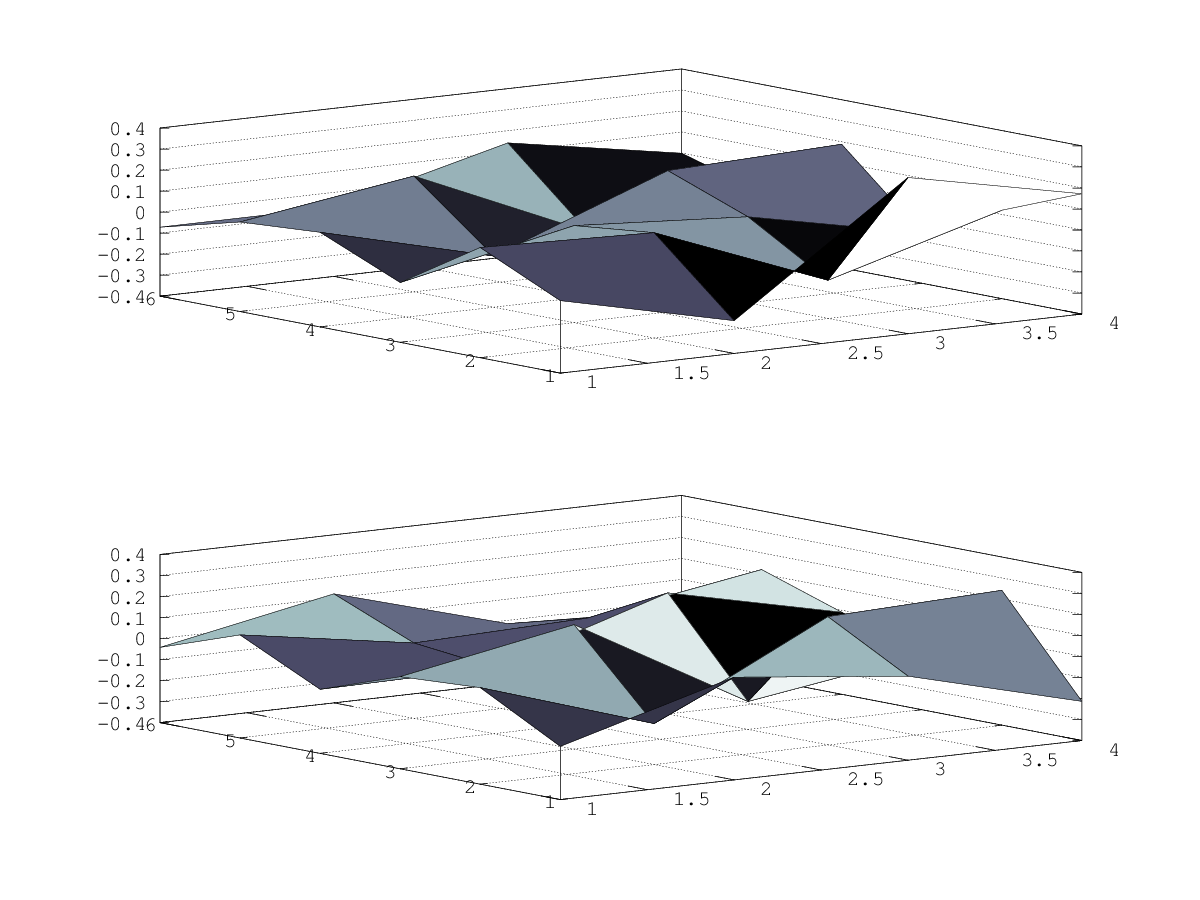
\includegraphics[scale=0.35]{/media/joe/Milarepa/Quall_Docs/miller/experiments/new_exp/05/trial10/figures/mode03}
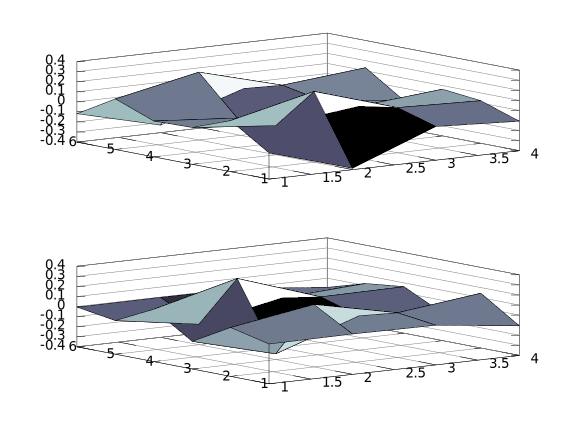
\includegraphics[scale=0.35]{/media/joe/Milarepa/Quall_Docs/miller/experiments/new_exp/05/trial10/figures/mode04}
\caption{(above) block 1, trial 10, pass 1, modes 3 \& 4}
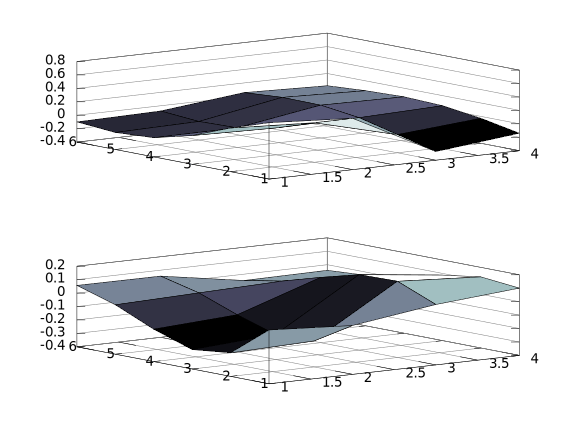
\includegraphics[scale=0.35]{/media/joe/Milarepa/Quall_Docs/miller/experiments/new_exp/05/trial10/figures/mode05}
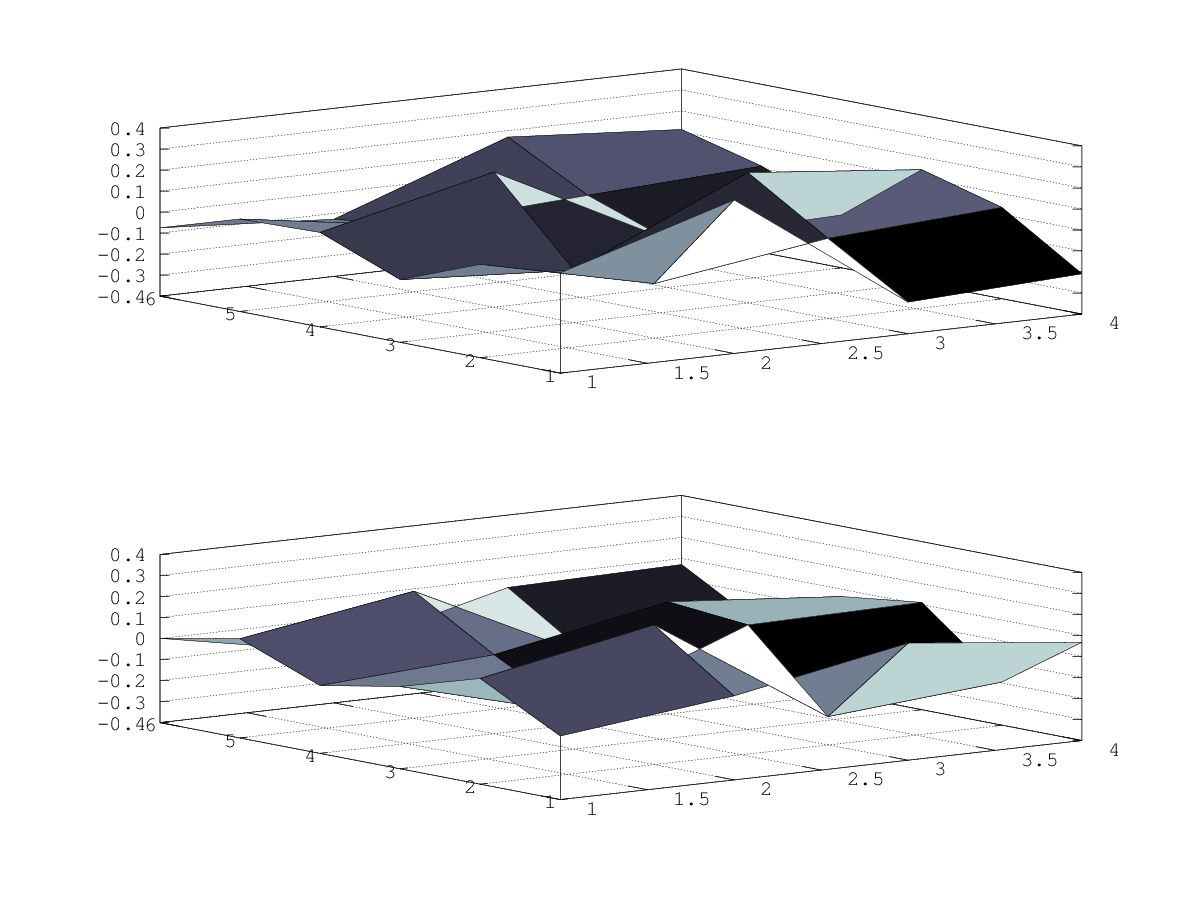
\includegraphics[scale=0.35]{/media/joe/Milarepa/Quall_Docs/miller/experiments/new_exp/05/trial10/figures/mode06}
\caption{(above) block 1, trial 10, pass 1, modes 5 \& 6}
\end{figure}
\begin{figure}[h]
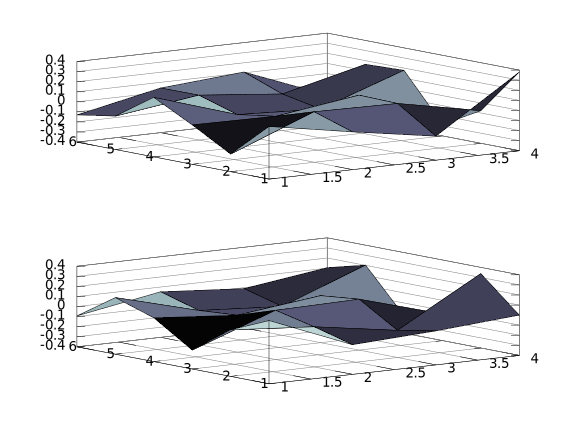
\includegraphics[scale=0.35]{/media/joe/Milarepa/Quall_Docs/miller/experiments/new_exp/05/trial10/figures/mode07}
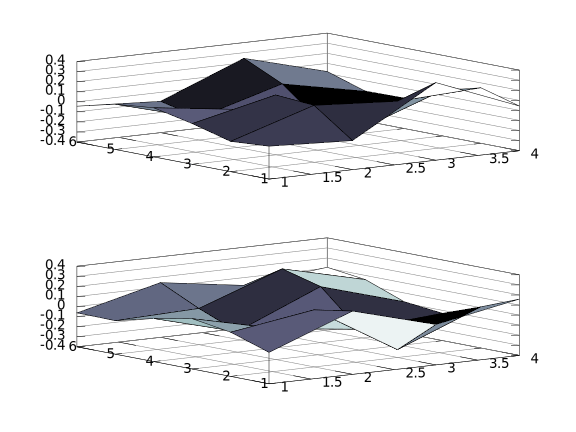
\includegraphics[scale=0.35]{/media/joe/Milarepa/Quall_Docs/miller/experiments/new_exp/05/trial10/figures/mode08}
\caption{(above) block 1, trial 10, pass 1, modes 7 \& 8}
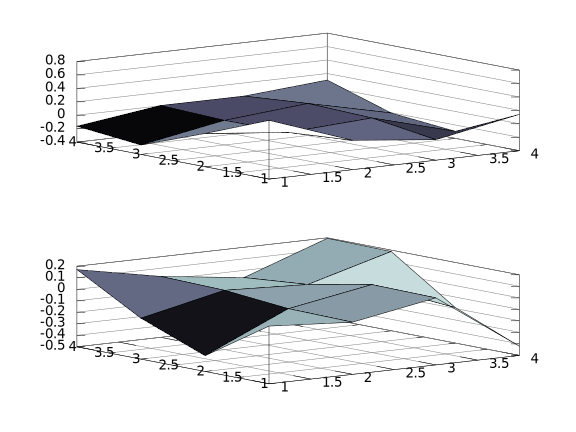
\includegraphics[scale=0.35]{/media/joe/Milarepa/Quall_Docs/miller/experiments/new_exp/05/trial10/figures/mode09}
\includegraphics[scale=0.35]{/media/joe/Milarepa/Quall_Docs/miller/experiments/new_exp/05/trial10/figures/mode10}
\caption{(above) block 1, trial 10, pass 1, modes 9 \& 10}
\includegraphics[scale=0.35]{/media/joe/Milarepa/Quall_Docs/miller/experiments/new_exp/05/trial10/figures/mode11}
\includegraphics[scale=0.35]{/media/joe/Milarepa/Quall_Docs/miller/experiments/new_exp/05/trial10/figures/mode12}
\caption{(above) block 1, trial 10, pass 1, modes 11 \& 12}
\end{figure}
\begin{figure}[h]
\includegraphics[scale=0.35]{/media/joe/Milarepa/Quall_Docs/miller/experiments/new_exp/05/trial10/figures/mode13}
\includegraphics[scale=0.35]{/media/joe/Milarepa/Quall_Docs/miller/experiments/new_exp/05/trial10/figures/mode14}
\caption{(above) block 1, trial 10, pass 1, modes 13 \& 14}
\includegraphics[scale=0.35]{/media/joe/Milarepa/Quall_Docs/miller/experiments/new_exp/05/trial10/figures/mode15}
\includegraphics[scale=0.35]{/media/joe/Milarepa/Quall_Docs/miller/experiments/new_exp/05/trial10/figures/mode16}
\caption{(above) block 1, trial 10, pass 1, modes 15 \& 16}
\includegraphics[scale=0.35]{/media/joe/Milarepa/Quall_Docs/miller/experiments/new_exp/05/trial10/figures/mode17}
\includegraphics[scale=0.35]{/media/joe/Milarepa/Quall_Docs/miller/experiments/new_exp/05/trial10/figures/mode18}
\caption{(above) block 1, trial 10, pass 1, modes 17 \& 18}
\end{figure}
\begin{figure}[h]
\includegraphics[scale=0.35]{/media/joe/Milarepa/Quall_Docs/miller/experiments/new_exp/05/trial10/figures/mode19}
\includegraphics[scale=0.35]{/media/joe/Milarepa/Quall_Docs/miller/experiments/new_exp/05/trial10/figures/mode20}
\caption{(above) block 1, trial 10, pass 1, modes 19 \& 20}
\includegraphics[scale=0.35]{/media/joe/Milarepa/Quall_Docs/miller/experiments/new_exp/05/trial10/figures/mode21}
\includegraphics[scale=0.35]{/media/joe/Milarepa/Quall_Docs/miller/experiments/new_exp/05/trial10/figures/mode22}
\caption{(above) block 1, trial 10, pass 1, modes 21 \& 22}
\includegraphics[scale=0.35]{/media/joe/Milarepa/Quall_Docs/miller/experiments/new_exp/05/trial10/figures/mode23}
\includegraphics[scale=0.35]{/media/joe/Milarepa/Quall_Docs/miller/experiments/new_exp/05/trial10/figures/mode24}
\caption{(above) block 1, trial 10, pass 1, modes 23 \& 24}
\end{figure}
\end{singlespace}
\end{section}
\end{chapter}

\begin{singlespace}
\bibliography{/media/joe/Milarepa/Quall_Docs/bibliography/qualls2}
\bibliographystyle{plain}
%\nocite{*}
\end{singlespace}
\end{document}
